\chapter{Tau Lepton Decay Modes Classification}
\label{chap:Tau}

\chapterquote{Give a man a fish and you feed him for a day; teach a man to fish and you feed him for a lifetime.}%
{}%: Blackwood's Magazine May 1830

The tau lepton has been studied extensively in the past at the Large Electron Positron Collider (LEP)\cite{Schael:2005am}. The tau lepton spin state, which can be derived from kinematic properties of its decay products, can be used to measure the CP (the product of charge conjugation and parity symmetries) of the Higgs, via \HiggsToTauTau channel\cite{Berge:2015nua}.  The polarisation correlation of the tau pairs can be used to infer the spin of the parent boson, differentiating \HiggsToTauTau from \ZToTauTau.

\begin{comment}
\FIGURE{fig:tauTheorySpin} shows an example of  difference in distributions for the two channels.
\begin{figure}[!htbp]
\centering
% \begin{center}/\end{center} takes some additional vertical space
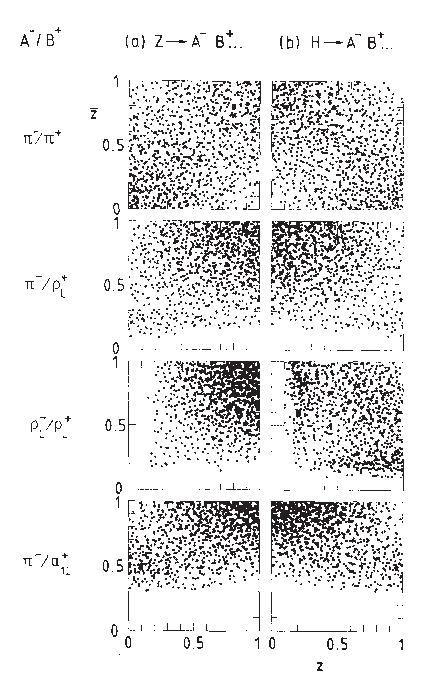
\includegraphics[width=.45\textwidth]{tau/theory}
\caption[An example of  difference in distributions for \HiggsToTauTau and \ZToTauTau.]
{
The two-dimensional distribution of (a) \HepProcess{\PZ \to \APtauon \Ptauon \to A^- B^+ \Pnut \APnut } (b) \HepProcess{\PHiggs \to \APtauon \Ptauon \to A^- B^+ \Pnut \APnut } events shown as functions of the energy fractions of $z = E_{A} / E_{\Ptauon}$ and $\overline{z} =  E_{B} / E_{\APtauon}$. In descending order the four sets of plots are for the (\APtauon, \Ptauon) pair decaying into (\Ppiminus, \Ppiplus), (\Ppiminus, $\rho_L^+$), ($\rho_L^-$, $\rho_L^+$) and finally (\Ppiminus, $a_{1L}^+$), each together with a \Pnut \APnut neutrino-pair. Plot is taken from \cite{Bullock:1991my}.
}
\label{fig:tauTheorySpin}
\end{figure}
\end{comment}

The ability to identify tau decay mode can also a benchmark for detector performance. Since tau lepton has a very short lifetime of 290\,fs \cite{Abreu:1991jn,Agashe:2014kda}, only its decay products can be detected with the tracking detectors and calorimeters. Therefore the performance of the calorimetric and track systems determines the ability to reconstruct the tau lepton decay products and identify different tau decay modes.


The main challenge in the tau lepton decay modes  classification is to reconstruct and separate spatially close photons. Many final states of the tau decay involves \Ppizero, where \HepProcess{\Ppizero \to \Pphoton \Pphoton}. For some final states, the one difference in the topology is the number of photons. At high centre-of-mass energy, the decay product of the tau decay are often boosted.  To reconstruct two photons from \Ppizero decay  separate entities requires good pattern recognition algorithms for photons and a \ECAL spatial resolution. Hence the photon reconstruction dedicated in \Chapter{chap:Photon} is used in this study to identify photons.

This chapter is organised as follows. Firstly, the analysis chain to identify tau decay modes will be described. The performance of the tau decay mode classification will be given, followed by the \ECAL optimisation study using the decay mode classification as a benchmark. Lastly, the  tau decay mode classification is further used in a proof-of-principle analysis to demonstrate the ability to identify \PHiggs from \PZ using  tau pair decay channel.

%
%The impact of the \ECAL transverse spatial resolution on the tau decay classification is demonstrated as well.



\section{Overview of the analysis}

The analysis starts with defining the samples for study in \Section{sec:tauDecayModes}. The seven major tau lepton decay modes are chosen for the classification. The simulation and reconstruction of these tau lepton decay are described in \Section{sec:tauSim}.  Pre-selection of the events, discussed in \Section{sec:tauPreSel}, are such that the reconstruction and detector effect, which do not vary with the \ECAL cell sizes, are not included in this analysis. After defining discriminative variables in \Section{sec:tauVar}, the classification is performed with a multivariate classifier. Since one decay mode needs to be classified into one of the seven decay modes, a multiclass classicisation is used to allow simultaneous classification between  multiple final states, which is presented in \Section{sec:tauMVA}.

The classification of the tau lepton decay modes are then  repeated for different energies of tau lepton decay to access the impact of the energy on classification. The classification is also used to study the effect of the \ECAL cell size on the classification performance. The impact of the tau energy and the \ECAL cell size on the classification performance is discussed in \Section{sec:tauECAL}. Lastly, the classification is utilised to demonstrate the ability to separate \PHiggs from \PZ using  tau pair decay channel in a proof-of-principle analysis, described in the \Section{sec:tauHZ}.

% The difference in the spin of the boson reflects in the different spin correlation of the tau pair. By extracting the spin correlation, parent bosons can be separated.
%This classification is repeated for different energies of tau lepton decay to access the impact of energy on classification. The impact of the \ECAL design is studied afterwards, where the \ECAL square cell size is varied. An overall tau hadronic decay classification efficiency is constructed to allow direct and easy comparison between different detector design and different energies of the tau decay.

% The study of the tau final state classification in the context for the  \ECAL optimisation allows the analysis to discard reconstruction and detector issue that do not vary with the \ECAL design. For example, the early photon conversion that happens in the tracking detector would complicate the event topology. But since it is affected by the tracker design, it can be ignored in this analysis. \SECTION{sec:tauSim}  and \Section{sec:tauPreSel} discuss the pre-selection cuts to choose the signal samples and events for this analysis.

%The classification is performed with a multivariate classifier. Discriminating variables are calculated before feeding into the classifier.  A multiclass classicisation is used to allow simultaneous classification between  multiple final states, described in \Section{}.


%A proof-of-principle analysis to demonstrate the ability to identify \PHiggs from \PZ using  tau pair decay channel is presented in the \Section{}. The difference in the spin of the boson reflects in the different spin correlation of the tau pair. By extracting the spin correlation, parent bosons can be separated.

%The follow sections on the analysis use the a 50\,GeV tau lepton decaying sample, reconstructed with nominal the \ILD detector model.

\section{Samples for the analysis}
\label{sec:tauDecayModes}

%\section{Select single tau decay}
The sample with simplest tau lepton decay in a \ee collider is chosen: \eeToTauTau. An example of the simulated \eeToTauTau event is shown in \Figure{fig:tauEvtDsp}. The \eeToTauTau channel contains two tau leptons travelling in opposite directions. Since the tau decay final state separation is applicable to a single tau lepton, particles in one event are divided into two collections. Each collection corresponds  to the decay products of one tau lepton.

The principle thrust axis vector is used to separation particles into two collections. Two collections are obtained based on the sign of the scalar product between the principle thrust axis vector  and the particle momentum vector. The classical event shape thrust, $T$,  \cite{PhysRevLett.39.1587}, is defined as
\begin{equation}
T = \max_{\hat{t}}\!\frac{\sum_{i}\absOf{\hat{t}\!\cdot\!\vec{p_{i}}}}{\sum_{i}\absOf{\vec{p_{i}}}}
\end{equation}
where $\vec{p_{i}}$ is the momentum vector of the particle $i$;   $\hat{t}$, is a unit principle thrust axis vector; and the summation is over all particles in an event. Thrust axis is useful to separate each jet in a back-to-back two-jet event.
%Thrust value, $T$, is 1 for a perfect pencillike back-to-back two-jet event, and 0.5 for a perfect spherical event. The thrust value is useful in picking out back-to-back two-jet event.


\begin{figure}[tbph]
\centering
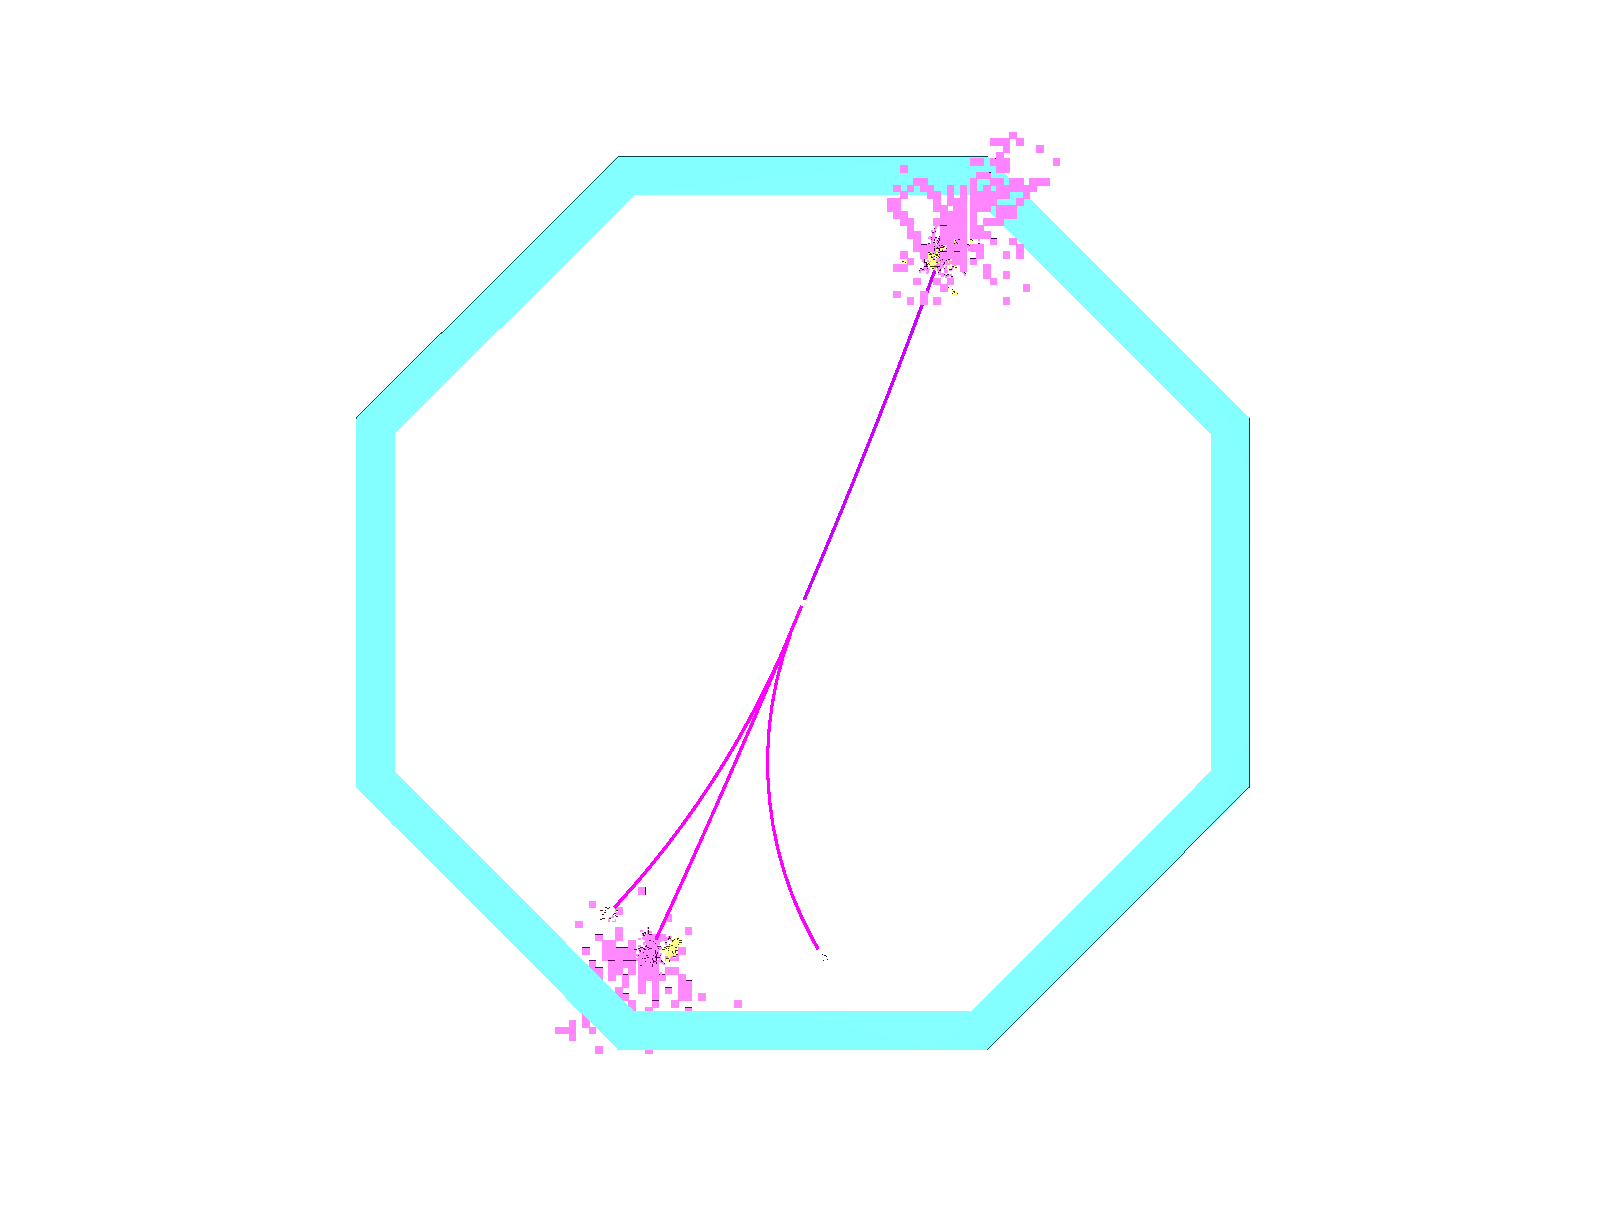
\includegraphics[width=0.65\textwidth]{tau/tau_evt_dsp2}
\caption{ An example event display of a simulated \eeToTauTau event using a \ILD detector model. The top half of the event is a tau lepton decaying into \decayRhoFinalStateShort final state and the bottom half of the event is a tau lepton decaying into  \decayThreePionPhotonShort final state. The purple lines are the tracks left by \Ppipm in the tracking detector. The purple clusters are the energy deposition by \Ppipm and the yellow clusters are the energy deposition by photon from \HepProcess{\Ppizero \to \Pphoton \Pphoton}. The blue region is the transverse cross section of the \ECAL barrel along the beam line direction.}
\label{fig:tauEvtDsp}
\end{figure}

\subsection{Tau lepton decay modes}

Tau lepton decays into a numerous number of final states. To study the predominant effect of the tau lepton decays, decay modes with branching ratio above 2\% are studied. This results in seven tau lepton decay modes. Their branching ratios, along with decay modes and final states are  shown in \Table{tab:TauDecayMode}. The seven tau lepton decay modes, which cover 92.58\,\% of all tau decay, are chosen to study in this analysis

% The most difficult final states to separate are \decayRhoFinalStateShort and \decayAiPhotonFinalStateShort, where photons from boosted \Ppizero are very challenging to reconstruct correctly.

\begin{table}[htbp]\centering
\smallskip
\begin{tabular}{l l r}
\hline
\hline
Decay modes & Detectable final states & Branching ratio\\
\hline
\decayElectron   &  \decayElectronShort  & $17.83\%_{\pm0.04\%}$   \\
\decayMuon &	\decayMuonShort & $17.41\%_{\pm0.04}$  \\
\decayPion  &   \decayPionShort	& $10.83\%_{\pm0.06}$   \\
\decayRho   & \decayRhoFinalStateShort& $25.52\%_{\pm0.09\%}$ \\
\decayAi   & \decayAiPhotonFinalStateShort	& $9.30\%_{\pm0.11\%}$    \\
\decayAi  &	\decayAiPionFinalStateShort    & $8.99\%_{\pm0.06\%}$  \\
\decayThreePionPhoton  &	\decayThreePionPhotonShort    & $2.70\%_{\pm0.08\%}$  \\
\hline
\hline
\end{tabular}
\caption[Decay modes, detectable final state particles and branching ratios of the seven major \Pgtm decays.]
{Decay modes, detectable final state particles and branching ratios of the seven major \Pgtm decays, taken from \cite{Agashe:2014kda}. \Pgtp decays similarly to \Pgtm.}
\label{tab:TauDecayMode}
\end{table}

\section{Simulation and reconstruction}
\label{sec:tauSim}

Two million \eeToTauTau events are simulated and reconstructed. The \ILD detector model was used. As the study is aimed for optimisation study of the \ECAL cell sizes, the beam specific effects does not vary with the \ECAL cell sizes are not simulated.  These effects include the initial state radiation (ISR) and the beam induced background.


The software used for simulation and reconstruction is described in \Chapter{chap:Reconstruction}. Events are reconstructed with  \ilcsoft version v01-17-07 \cite{Gaede:82475} and \pandora version 3 \cite{Marshall:2015rfa}, where the photon reconstruction is discussed in \Chapter{chap:Photon}.


\section{Event pre-selection}
\label{sec:tauPreSel}

Since the analysis is aimed for the optimisation of the \ECAL cell sizes, pre-selection cuts that are not affected by the \ECAL cell sizes are used. These cuts also allow the analysis to focus on the events with clear topologies. The pre-selection cuts are listed in \Table{tab:tauPreSel}. The fraction of events passing each pre-selection cut for individual decay mode are listed in \Table{tab:tauPreSelEff}.

One of the pre-selection cuts is to demand that the event does not have photons converted to electron pairs in the tracking detector. These discarded events would have few photons and more electrons in the final states, which changes the topologies of the final states. Shown in \Table{tab:tauPreSelEff}, only decay modes with photons in the final states are affected by this cut, as expected.


Another pre-selection cut is the total energy of the non-neutrinos tau decay products, $E_{vis,MC}$, > 5\,GeV, based on the truth information. If most energy of the tau lepton is carried by the neutrinos, it is difficult to identify the low-energy non-neutrino tau decay products. Hence these events with low energy of the non-neutrinos tau decay products are not used in the analysis. Decay modes with only one non-neutrino particle in the final states are mostly affected by this cut, indicated in \Table{tab:tauPreSelEff}.

The last pre-selection cut is to avoid events with energy deposition in the gap region between barrel and the end cap part of the calorimeter. As the reconstruction   does not attempt to recover reconstruction in the gap region, threw is a significant drop in the particle reconstruction efficiency. The cut demands the absolute value of the polar angle of tau lepton,  $\absOf{\theta_{Z,MC}}$, based on the truth information, is between 0.3 and 0.6\,rad to be contained in the end cap region, or is between 0.8 and 1.57 to be contained in the barrel region. All decay modes are affected almost equally by this cut, suggested by the numbers in \Table{tab:tauPreSelEff}.


\begin{table}[htbp]\centering
\smallskip
\begin{tabular}{l r}
\hline
\hline
Cuts & Values\\
\hline
\multicolumn{1}{L{0.4\textwidth}}{Photon conversion in the tracking detector}& No \\
\multicolumn{1}{L{0.4\textwidth}}{Total energy of non-neutrino decay products} & $E_{vis,MC} > 5\,GeV$ \\
Polar angle acceptance & \multicolumn{1}{R{0.5\textwidth}}{$0.6 > \absOf{\theta_{Z,MC}} > 0.3$ or $1.57 > \absOf{\theta_{Z,MC}} > 0.8$} \\
\hline
\hline
\end{tabular}
\caption[Pre-selection cuts for tau lepton decay final state classification.]
{Pre-selection cuts for tau lepton decay modes classification.}
\label{tab:tauPreSel}
\end{table}


\begin{table}[htbp]\centering
\smallskip
\begin{tabular}{ l r r r}
\hline
\hline
 \multicolumn{1}{R{0.2\textwidth}}{Detectable final state}   & \multicolumn{1}{R{0.25\textwidth}}{No photon conversion in the tracking detector} & \multicolumn{1}{R{0.25\textwidth}}{Total energy of non-neutrino decay products acceptance} &\multicolumn{1}{R{0.25\textwidth}}{Polar angle acceptance} \\
\hline
\decayElectronShort& 100.0\% & 84.7\%& 66.2\%\\
\decayMuonShort &100.0\%& 85.2\%&66.7\%\\
\decayPionShort &100.0\%& 88.3\%&60.9\%\\
\decayRhoFinalStateShort &77.1\%&76.9\%&61.9\%\\
\decayAiPhotonFinalStateShort &61.3\%&61.2\%&50.5\%\\
\decayAiPionFinalStateShort &100.0\%&100.0\%&78.0\%\\
\decayThreePionPhotonShort &77.0\%&77.0\%&61.8\%\\
\hline
\hline
\end{tabular}
\caption
{The fraction of events passing each pre-selection cut for individual decay mode. Cuts are presented in a ``flow'' fashion, where each column contains all the cuts to its left.}
\label{tab:tauPreSelEff}
\end{table}

%The no photon early conversion cuts only effective against final states with \Ppizero, as \Ppizero decays to a photon pair. For final states with one \Ppizero, about 77\% events survived. For final states with two \Ppizero, about 61\% events survived, which is roughly $0.77^2$. For the visible angle acceptance, final states with only one particle are affected the most, whilst final states with more than one particles typically have more visible energies. The polar angle acceptance efficiencies depend on the final states, as light final states are boosted and more likely in the forward region.



%An low visible energy event is discarded if the total energy of the tau lepton visible decay products is below 5\,GeV. Requirement of the tau decay in the barrel or the end cap part of the calorimeter is defined as the polar angle of the tau is $ 17.2\degree < |\theta_{Z}| < 34.4\degree$ or $ 45.8\degree < |\theta_{Z}| < 90\degree$.





\section{Variables used in the MVA}
\label{sec:tauVar}


Having pre-selected events, discriminating variables are carefully developed for the multivariate analysis (MVA). The full list of the variables are shown in \Table{tab:tauVaraibles}. The distribution of the four most power variables are shown in \Figrure{fig:tauVar}.



The most crucial variables are the number of \PFOs of different particles. \FIGURE{fig:tauVarNCharge} shows the distribution of ${N}_{\charge}$, the number of  charged \PFOs for different tau final states. Whilst over 98\% 1-prong final states have one track reconstructed, around 95\%  3-prong final states have three tracks reconstructed. This is an excellent variable to separate 1-prong and 3-prong final states. An orthogonal measurement is the number of reconstructed photons,  ${N}_{\Pgg}$, shown in \Figure{fig:tauVarNPhoton}. The overlap between \decayPionShort and \decayRhoShort final states is about 15\% and the confusion between \decayRhoShort and \decayAiPhotonShort is around 15\%. ${N}_{\Pgg}$ can also separate two 3-prong final states. ${N}_{\Pmu}$, ${N}_{\Pe}$, ${N}_{\Pgpm}$ are useful to identify two leptonic final states, and further separate 3-prong final states from 1-prong final states.

Invariant masses of different particles are good at characterising different final states. \FIGURE{fig:tauVarMVis} shows the invariant mass of the system. Clear reasonable peaks can be seen for \Prho and \Pai. The mass peak of  \decayAiPionFinalStateShort are much higher. $m_{\charge}$ and $m_{\neutral}$ are invariant masses of charged and neutral particles respectively. They separate final states with neutral particles from those without neutral particles. Similarly, $m_{\Pgg}$ and $m_{\Pgpm}$ identify final states with photons and with \Pgpm respectively.

Calorimetric information is used to identify electron and muon. An electron deposits most energy in the \ECAL and a muon deposits 5 to 20\% energy in the \ECAL. Two variables, $\% E_{\charge}$ and $\% E$, are the fraction of energy deposited in the \ECAL over total energy in the calorimeter, of charged particles and all \PFOs respectively. Energy fraction for the charged particles does not include contribution from photons, which also deposit most energy in the \ECAL, like electrons.

Energy information further separate different final states. Variables are normalised to the expect tau energy. For example, $\tilde{E}_{\Pgg}$, normalised energy of photons are different for final states with and without photons.

Extra variables are used to differentiate specific final states.

\subsection{\texorpdfstring{\decayRhoShort and \decayRhoShort} \, resonances reconstruction}
\label{sec:tauResonance}
\decayRhoShort and \decayAiPhotonShort are identified further using their resonance structure. For example, \decayRhoShort final state contains a \Pgpm and a \Ppizero decaying to two photons. By selecting \Pgpm and photons consistent with \Prho decay pattern, \decayRhoShort final state could be separated. The particle selection is via minimising a  $\chi^{2}$ function, defined as:
\begin{equation}
\chi^{2} = {\left(\frac{m_{tot} -  m^{MC}_{\Prho}}{\sigma^{MC}_{\Prho}}\right)}^{2} + {\left(\frac{m_{\Pphoton \Pphoton} -  m^{MC}_{\Ppizero}}{\sigma^{MC}_{\Ppizero}}\right)}^{2} \,,
\end{equation}
where $m_{\Pphoton \Pphoton}$ is the invariant mass of two photons and $m_{tot}$ is the invariant mass of the  photon pair and one \Pgpm. All combinations of photons and \Pgpm are tested. $m^{MC}_{\Prho}$ and $m^{MC}_{\Ppizero}$ are expected masses of \Prho and \Ppizero, taken from \cite{Agashe:2014kda}. $\sigma^{MC}_{\Prho}$ and $m^{MC}_{\Ppizero}$ are the half width of the invariant mass distribution of reconstructed \Prho and \Ppizero using the truth information. This minimisation allows \decayRhoShort final state to be separated from \decayAiPhotonShort, where failure to reconstruct photons causes  \decayAiPhotonShort events to be simualr to that of \decayRhoShort.

Similarly, \decayAiPhotonShort can be separate using a extended minimisation with two extra photons:
\begin{equation}
\chi^{2} = {\left(\frac{m_{tot} -  m^{MC}_{\Pai}}{\sigma^{MC}_{\Pai}}\right)}^{2} + {\left(\frac{m_{\Pphoton1 \Pphoton2} -  m^{MC}_{\Ppizero}}{\sigma^{MC}_{\Ppizero}}\right)}^{2}  + {\left(\frac{m_{\Pphoton3 \Pphoton4} -  m^{MC}_{\Ppizero}}{\sigma^{MC}_{\Ppizero}}\right)}^{2} \,,
\end{equation}
where \Prho has been replace by \Pai. Selected particles for the test are two photon pairs and one \Pgpm. Both photon pairs are required to be consistent with \Ppizero decaying to two photons. \FIGURE{fig:tauVarMA1} shows the distribution of $m_{tot}$ from \decayAiPhotonShort consistency test for selected final states. The main feature is that only \decayAiPhotonShort final state has a mass peak at \Pai resonance position. Comparing to simple invariant mass distribution in \Figure{fig:tauVarMVis}, \decayAiPhotonShort mass peak is enhanced.

The $\chi^{2}$ functions for both consistency test are adapted for cases where reconstruction fails to resolve photon pairs. Relevant terms are dropped from the expression if there are fewer photons than required.

\subsection{Separate \decayElectronShort from \decayPionShort}

Particle ID reported from \pandora is used extensively to reconstruct discriminating variables. \pandora uses a wide range of information to determine electron ID. However, extra information is used in this analysis to help identifying electrons, which are mistaken as \Pgpm by \pandora reconstruction.

An electron leaves a characteristic electromagnetic  (EM) shower in the \ECAL (see \Section{sec:photonEMshower}), whilst \Pgpm doesn't. Variables defining the  EM shower helps to identify \Pem, taken from photon reconstruction in \Section{sec:photonLikelihood}. $t_0$, the start layer of the longitudinal shower and $\delta{l}$, the fractional difference between observed and expected longitudinal shower profile describe the longitudinal EM shower. $\langle{w}\rangle$ is a measure of the EM shower transverse width.

Another type of information to differentiate an EM shower from a \Pem and a early hadronic shower from a \Pgpm is the calorimeter hit information. $\bar{E}_{hit}$, the average energy of a hit, and $\%MIP$, fraction of possible minimum ionising particles, are different for EM and hadronic showers. Last information used is the track-calorimeter consistency check. $\Delta E/P$ is the calorimeter energy divided by the track momentum. This variable is found to help to differentiate \decayElectronShort from \decayPionShort final state.



\begin{figure}[htbp]
\centering
% \begin{center}/\end{center} takes some additional vertical space
\begin{subfigure}[b]{0.45\textwidth}
 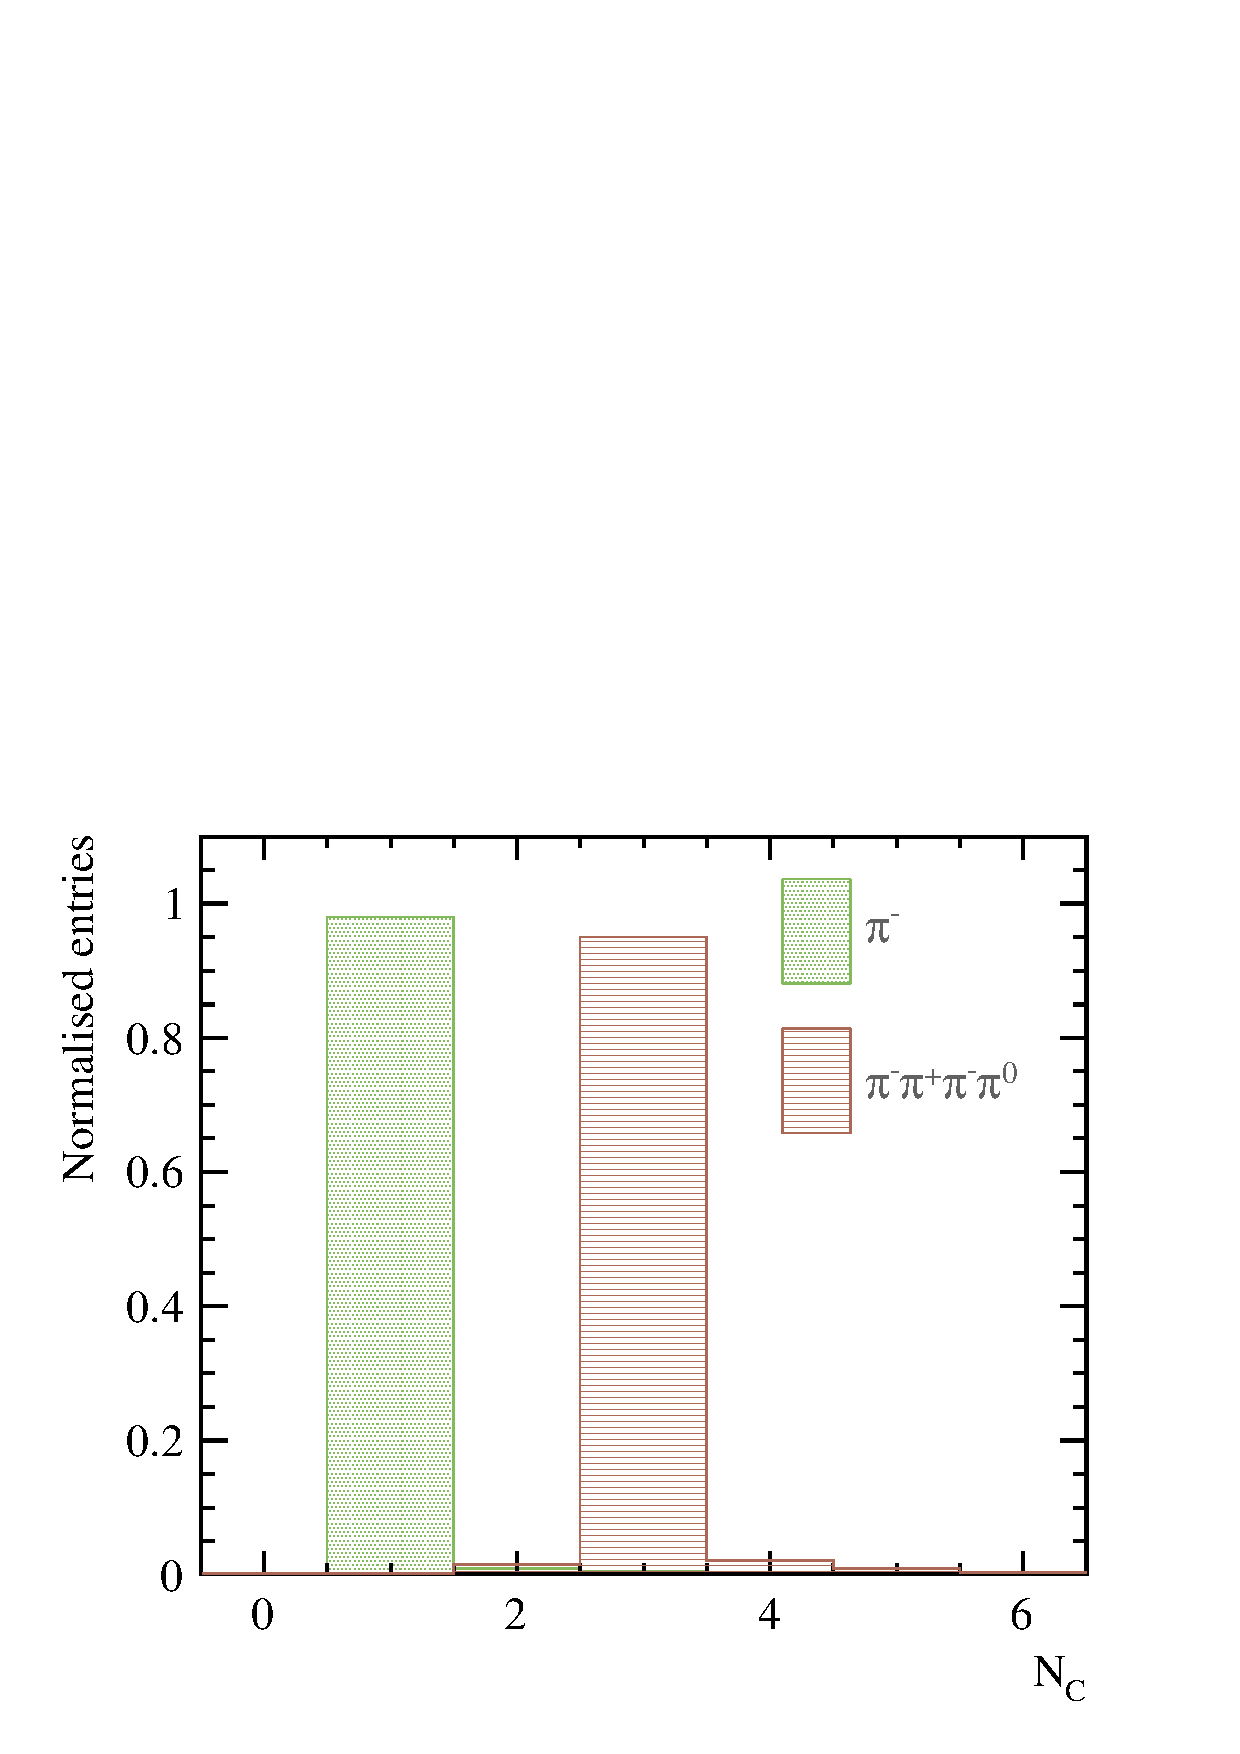
\includegraphics[width=\textwidth]{tau/var2/nCharge_100GeV_improved.pdf}
  \caption{}
  \label{fig:tauVarNCharge}
\end{subfigure}
\begin{subfigure}[b]{0.45\textwidth}
 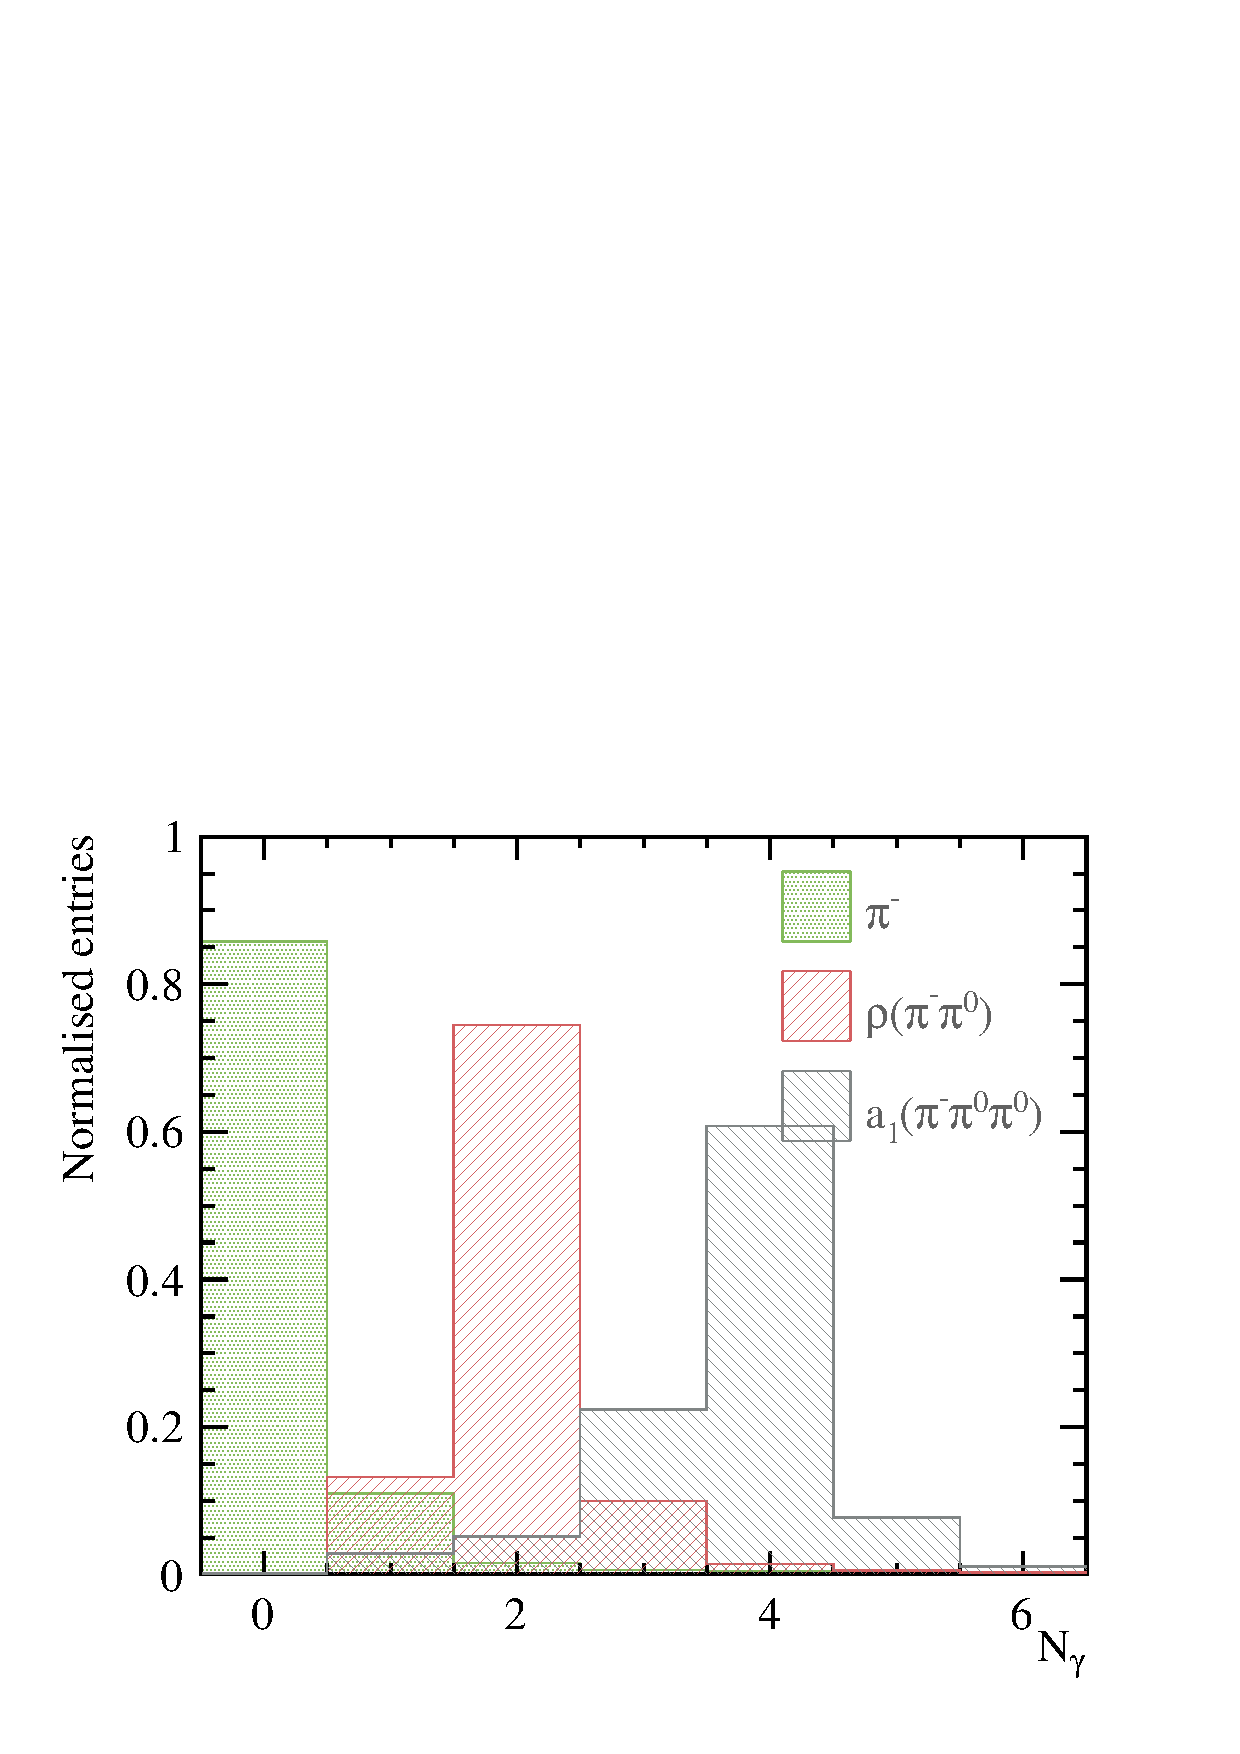
\includegraphics[width=\textwidth]{tau/var2/nPhoton_100GeV_improved.pdf}
  \caption{}
  \label{fig:tauVarNPhoton}
\end{subfigure}
\begin{subfigure}[b]{0.45\textwidth}
 \includegraphics[width=\textwidth]{tau/var2/mVis_100GeV_improved_zoom.pdf}
  \caption{}
  \label{fig:tauVarMVis}
\end{subfigure}
\begin{subfigure}[b]{0.45\textwidth}
 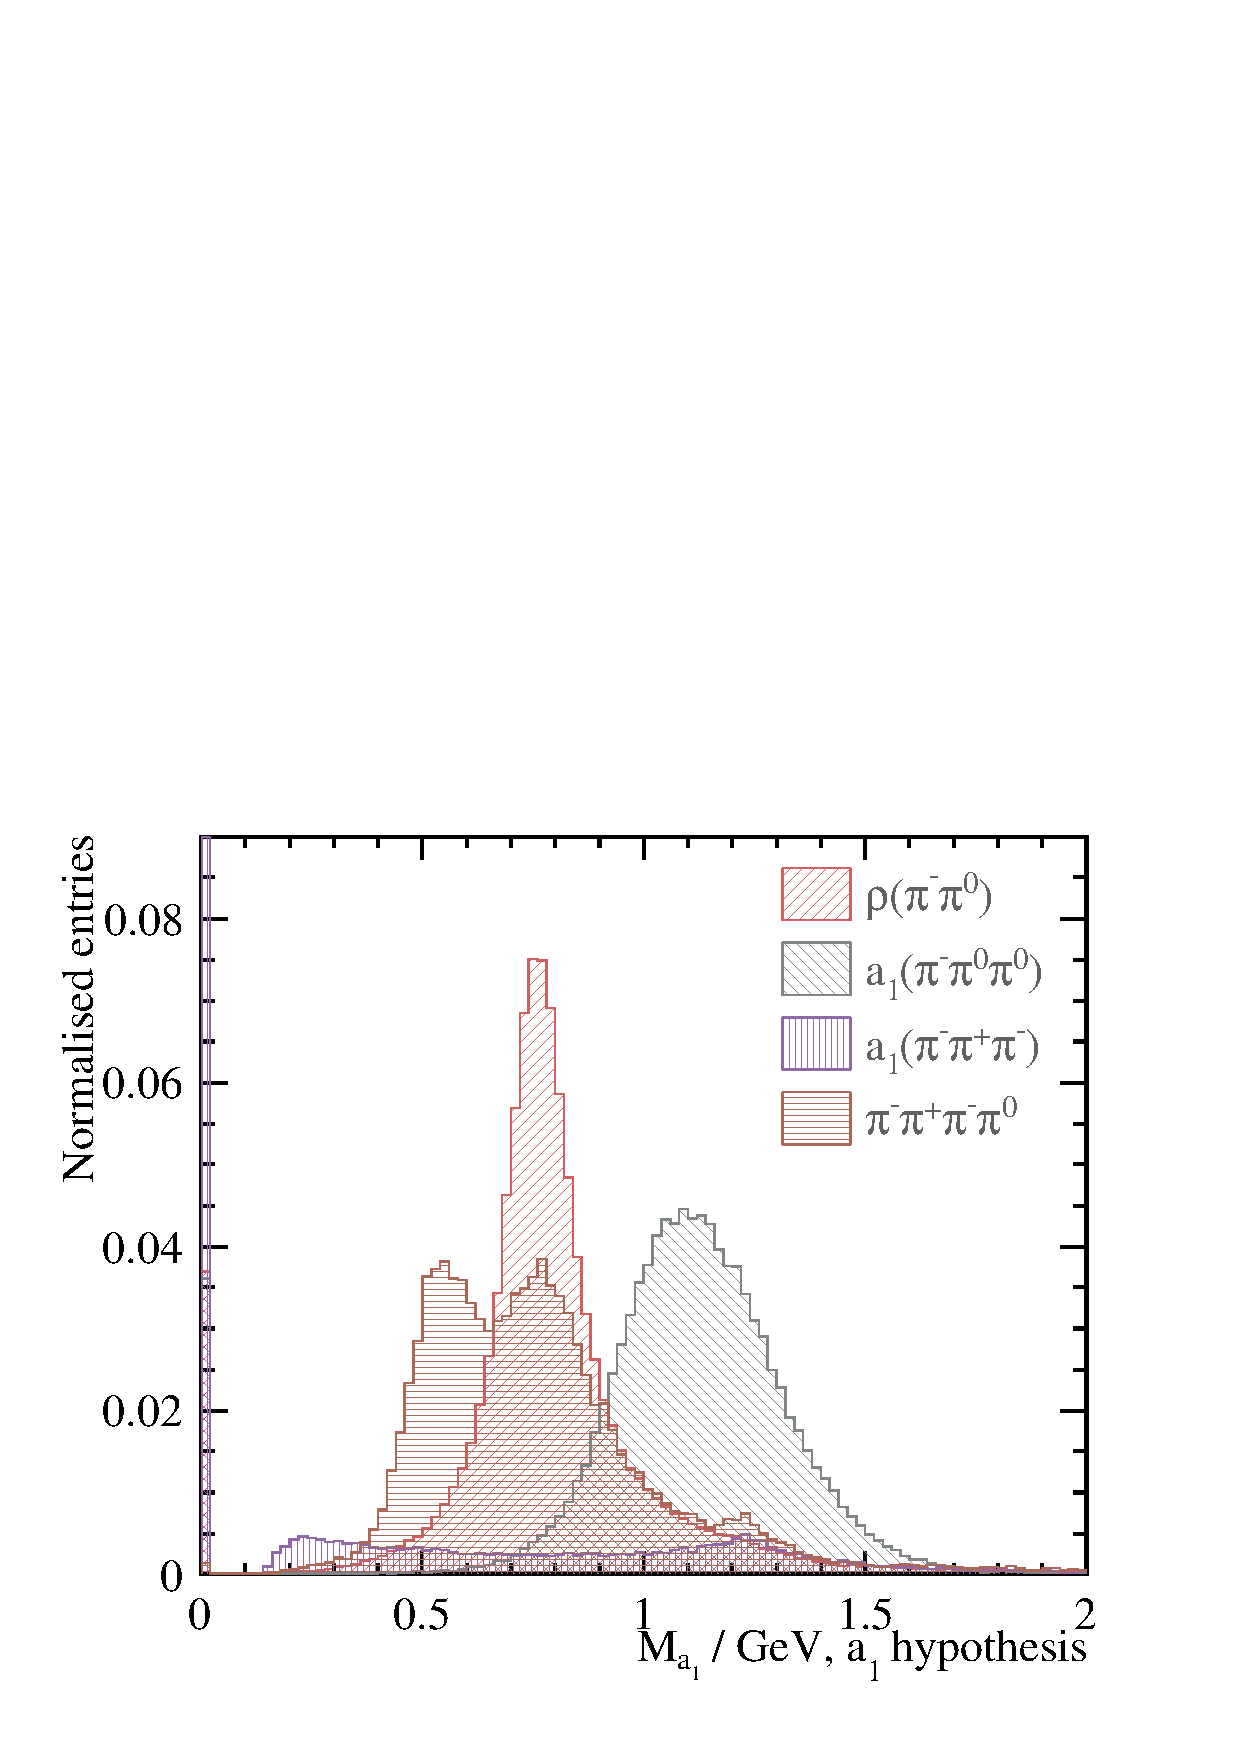
\includegraphics[width=\textwidth]{tau/var2/mA1A1Fit_100GeV_improved_zoom.pdf}
  \caption{}
  \label{fig:tauVarMA1}
\end{subfigure}

\caption
{Normalised distribution for a) the number of charged particle (${N}_{\charge}$)
 selected variables showing for seven final states, \decayElectronShort, \decayMuonShort, \decayPionShort, \decayRhoShort, \decayAiPhotonShort, \decayAiPionShort and \decayThreePionPhotonShort, separated using truth information. \FIGURE{fig:tauVarNCharge}, \Figure{fig:tauVarNPhoton}, \Figure{fig:tauVarMVis}, and \Figure{fig:tauVarMA1} show distributions for the number of tracks, the number of photons, the invariant mass of visible \PFOs, and the invariant mass of $a_1$ for \decayAiPhotonShort hypothesis test, respectively. The area for each final state is normalised to 1.
}
\label{fig:tauVar}
\end{figure}

\begin{table}[!htbp]\centering
\begin{tabular}{lr}
\hline
\hline
Category &  Variable \\
\hline
Number of \PFOs & \multicolumn{1}{R{0.6\textwidth}}{  ${N}_{\charge}$, ${N}_{\Pmu}$, ${N}_{\Pe}$, ${N}_{\Pgg}$,  ${N}_{\Pgpm}$} \\
Invariant mass &  \multicolumn{1}{R{0.6\textwidth}}{$m_{vis}$, $m_{\charge}$, $m_{\neutral}$, $m_{\Pgg}$, $m_{\Pgpm}$} \\
Calorimetric info. &   \multicolumn{1}{R{0.6\textwidth}}{ $\% E_{\charge}$,  $\% E$ } \\
Energy & \multicolumn{1}{R{0.6\textwidth}}{ $\tilde{E}_{vis}$,  $\tilde{E}_{\charge}$, $\tilde{E}_{\Pmu}$, $\tilde{E}_{\Pe}$, $\tilde{E}_{\Pgg}$,  $\tilde{E}_{\Pgpm}$} \\
\decayRhoShort reconstruction & \multicolumn{1}{R{0.6\textwidth}}{  $m_{\Pgpz}\parenths{\rho}$, $m_\rho$} \\
\decayAiPhotonShort reconstruction &  \multicolumn{1}{R{0.6\textwidth}}{  $m_{\Pgpz}\parenths{\Pai}$, $m^*_{\Pgpz}\parenths{\Pai}$, $m_{\Pai}$} \\
EM shower profile & $\delta{l}$, $t_0$, $\langle{w}\rangle$ \\
Calorimeter hit info. & $\bar{E}_{hit}$, $\%MIP$ \\
Track info. & $\Delta E/P$ \\
\hline
\hline
\end{tabular}
\caption
{Variables used in the MVA event selection for the tau lepton decay mode classification.}
\label{tab:tauVaraibles}
\end{table}

\section{Multivariate Analysis}
\label{sec:tauMVA}
For the multivariate analysis, the multiclass class of the TMVA package \cite{Therhaag:2009dp} was used to perform a multiclass classification, which trains the seven final states simultaneously. The multiclass class is an extension of the standard two-class signal-background classifier. The discussion on multivariate analysis can be found in \Section{sec:pandoraMVA}. The multiclass classifier is discussed in \Section{sec:pandoraMVAmulticlass}.

The multiclass classifier used is Boosted Decision Tree with Gradient boost (BDTG). The optimisation of the BDTG classifier follows the strategy in \Section{sec:pandoraMVAoptimisation}. The optimised parameters are listed in \Table{tab:tauBDTparameters}. Explanation of variables can be found in \Section{sec:pandoraMVAbdtVar}.  Half of the randomly selected samples were used in the training process and the other half were used for testing.

\begin{table}[!tbp]\centering
%\small
\begin{tabular}{lr}
\hline \hline
 Parameter &  Value \\
\hline
Depth of tree & 5 \\
Number of trees & 3000 \\
Boosting & gradient boost \\
learning rate of the gradient boost & 0.1 \\
metric for the optimal cuts & Gini Index \\
bagging fraction & 0.5 \\
Number of bins per variables & 100 \\
End node output & yes/no \\
\hline \hline
\end{tabular}

\caption
{Optimised parameters for the Boosted Decision Tree with Gradient boost multiclass classifier. See \Section{sec:pandoraMVAbdtVar} for detailed explanation of variables.}
\label{tab:tauBDTparameters}
\end{table}


\section{Classification Efficiency}

The reconstruction efficiencies for the seven tau decay final states are shown in \Table{tab:TauSelExample}. Bold numbers show the correct classification probability. For example, 99.8\%  of true \decayElectronShort are reconstructed correctly.

For the \decayElectronShort decay mode, a high correct classicisation is achieve, due to using particle ID from \pandora and calorimetric information. Similarly for \decayMuonShort decay mode,  99.5\% correct rate is achieved, due to efficient tracking detector and muon reconstruction algorithm.

For the \decayPionShort decay mode, 3.4\% confusion with \decayRhoShortest decay mode  is to due to differentiate two event topologies. Around 15\% of \decayPionShort events have at least one photon reconstructed, mostly due to the FSR. If the reconstruction is unable to identify the photon pair from \Ppizero decay in \decayRhoShortest decay mode, two decay modes would appear to  similar and confusion is caused. The confusion with \decayElectronShort is at percent level, which is low due to the usage of EM shower variables. The percent level confusion with \decayAiPionShortest is because the tracking efficiency is at 98\%, where 2\% \decayPionShort events have more than one track reconstructed.

For the \decayRhoShortest decay mode, biggest confusion is with \decayAiPhotonShortest because of the similar reason of unable to reconstruct all photons form \Ppizero decaying.

For the \decayAiPhotonShortest decay mode, the correct classicisation rate is the lowest as it is most challenging to reconstruct correctly: two photon pairs and  one \Ppipm. The 9.5\% confusion with \decayRhoShortest is due to the same reconstruction failure issue. It should be noted that \Figure{fig:tauVarNPhoton} suggests that 30\% of \decayAiPhotonShortest events have fewer than four photons reconstructed, which overlap with \decayRhoShortest distribution. The \decayAiPhotonShortest resonance reconstruction (\Section{sec:tauResonance}) and the multiclass classifier reduce the confusion to  9.5\% from 30\%.

For the \decayAiPionShortest decay mode, most confusion is with \decayThreePionPhotonShort, due to inability of separating photons. And the reason is the same for the confusion of  \decayThreePionPhotonShort decay mode classified as \decayAiPionShortest decay mode.
The unprecedented high classification rate has been achieved. The improvement of photon reconstruction described in \Section{} improved the ability to separate 1-prong final state. Most notably,  \Figure{} shows number of photons have a high correct reconstruction efficiency.


\begin{table}[htbp]
\centering
\small
%\smallskip
\begin{tabular}{ l   r  r  r  r  r  r  r }
\hline
\hline
Reco $\downarrow$ Truth $\to$  & \decayElectronShort & \decayMuonShort &\decayPionShort & \decayRhoShortest &\decayAiPhotonShortest &\decayAiPionShortest &\decayThreePionPhotonShort \\
\hline

{\decayElectronShort}&\textbf{99.7}&-&0.9&0.6&0.4&-&-\\
{\decayMuonShort}&-&\textbf{99.5}&0.6&-&-&-&-\\
{\decayPionShort}&-&0.3&\textbf{94.0}&0.8&-&0.4&-\\
{\decayRhoShort}&-&-&3.4&\textbf{93.6}&9.5&0.6&2.3\\
{\decayAiPhotonShort}&-&-&-&4.5&\textbf{89.7}&-&0.6\\
{\decayAiPionShort}&-&-&0.9&-&-&\textbf{96.8}&6.4\\
{\decayThreePionPhotonShort}&-&-&-&0.3&-&2.0&\textbf{90.6}\\

\hline
\hline
\end{tabular}

\caption[Classification efficiency for tau decay modes.]
{ Classification efficiency in percentage for tau decay modes using the nominal ILD detector model , for \rootSGeV{100}. Bold numbers show the correct classification probability. Numbers below 0.25\%, and \Pgngt are not shown in decay modes, for display purposes. Statistical uncertainties are less than 0.25\%.}
\label{tab:TauSelExample}
\end{table}




\section{Electromagnetic calorimeter  optimisation}
\label{sec:tauECAL}
In the above section, an analysis on tau decay mode classification is presented. Events are \eeToTauTau at \rootSGeV{100} with nominal \ILD detector model. This classification can be applied for different  \sqrtS and with different detector models. The main reconstruction issue is to separate boosted photon pair from \Ppizero decay. High \sqrtS would photon pair more collimated, and therefore more challenging to separate. The \ECAL cell size is crucial in separating the EM showers from photons. As discussed in previous chapter, separating photons requires a high transverse spatial resolution. Therefore, the \ECAL square cell size is expected to affect the classification efficiency.

The main difficulty in the classification is to classify 1-prong final states.  These final states involves \Ppizero, where two photons from \Ppizero decay could be poorly reconstructed. At high energy, \Ppizero is boosted making the reconstruction more challenging. The ability to reconstruct the two photons as separate entities requires good pattern recognition algorithm for photons and \ECAL spatial resolution. Hence the improved photon reconstruction in \Chapter{chap:Photon} is used in this study. The impact of the \ECAL transverse spatial resolution on the tau decay classification is demonstrated as well.

The analysis is repeated with varying \ECAL square cell sizes at 3, 5, 7, 10, 15 and 20\,mm, at four  \sqrtS = 100, 200, 500, 1000\,GeV. The multivariate classifier is trained for each cell size and each \sqrtS. Other \ECAL dimensions are kept the same as the \ILD nominal detector. Because the lepton reconstruction mostly relies on the tracking system, which is not varied in this study, only the  hadronic tau decays were investigated and compared between different \ECAL square cell sizes.


As \pandora is optimised for the nominal \ILD detector, fragment removal algorithms have a large dependence on the \ECAL cell sizes. One algorithm is re-optimised for the varying \ECAL cell sizes. The \PhotonFragmentRemoval algorithm which merges photon fragments uses a distance metric and it is optimised with values listed in the \Table{tab:TauPhotonFragmentRemovalParameter}. As cell sizes become larger, the distance cut for merging photons are larger.



\begin{table}[htbp]
\centering
%\small
%\smallskip
\begin{tabular}{ l   r  r  r  r  r  r  }
\hline
\hline
\ECAL square cell size (mm) & 3 & 5 & 7 & 10 & 15 & 20  \\
\hline
ClosestHitDistance & 5 & 10 & 10 & 10 & 20 & 20 \\
\hline
\hline
\end{tabular}

\caption[Optimised parameters of \PhotonFragmentRemoval algorithm as a function of \ECAL square cell size.]
{Optimised parameters of \PhotonFragmentRemoval algorithm as a function of \ECAL square cell size.}
\label{tab:TauPhotonFragmentRemovalParameter}
\end{table}


\FIGURE{fig:TauPionEfficiency} shows the correct classification efficiencies for  tau hadronic decay final states  as a function of the \ECAL square cell sizes. For example, plotted values for 5\,mm cell size at \rootSGeV{100} are the same as the bold numbers in \Table{tab:TauSelExample}.

In general,  the correct classification efficiencies generally decreases with increase of \sqrtS and increase of \ECAL cell sizes. As the \sqrtS increases, tau decay products are boosted. It is increasingly difficult to separate identical decay products. For example, the photon pair from \Ppizero decay become very challenging to separate at high \sqrtS. Increase of the \ECAL cell sizes has a similar effect. With a bigger cell size, photons may deposit energy in a same cell, making separating these photons  almost impossible.

For the \decayPionShort decay mode, the general trend is followed. The efficiency for \rootSGeV{200} is slightly better than that of the \rootSGeV{100} for small cell sizes.

For the \decayRhoShort decay mode,the efficiency for  \rootSGeV{500} increases as the cell sizes increases. This is because the multivariate classifier optimises for the overall classification efficiency, which may compensate one decay mode for another. In this case, the small increase in efficiency for \decayRhoShort at \rootSGeV{500} is compensated by the drastic decrease in efficiency for \decayAiPhotonShort at  \rootSGeV{500}.

For the \decayAiPhotonShort decay mode, the loss of efficiency with increase of the cell size and increase in \sqrtS is most significant comparing to other decay modes. With most number of particles in the final state, it is the most challenging decay channel to reconstruct and thus most sensitive to the change in cell sizes and \sqrtS.

For the \decayAiPionShort decay mode, the efficiencies are similar to that of the \decayPionShort. Both final states contain charged particles only. Therefore it is most sensitive to the tracking performance, which is not affected by the \ECAL cell sizes.

For the \decayThreePionPhotonShort decay mode, the decrease in efficiencies are more significant for \rootS{500} and 1000\,GeV.

The leptonic decay  correct reconstruction efficiency is not used as a metric as they are similar across different \ECAL cell sizes. This is because the \Pepm and \Pgmpm identifications mostly rely on the tracking system, which was not varied in this study. The energy deposited in the calorimeter are used for the association to the tracks but it has a small impact on the lepton identification.


\begin{figure}[htbp]
\centering % \begin{center}/\end{center} takes some additional vertical space
\begin{subfigure}[b]{0.45\textwidth}
  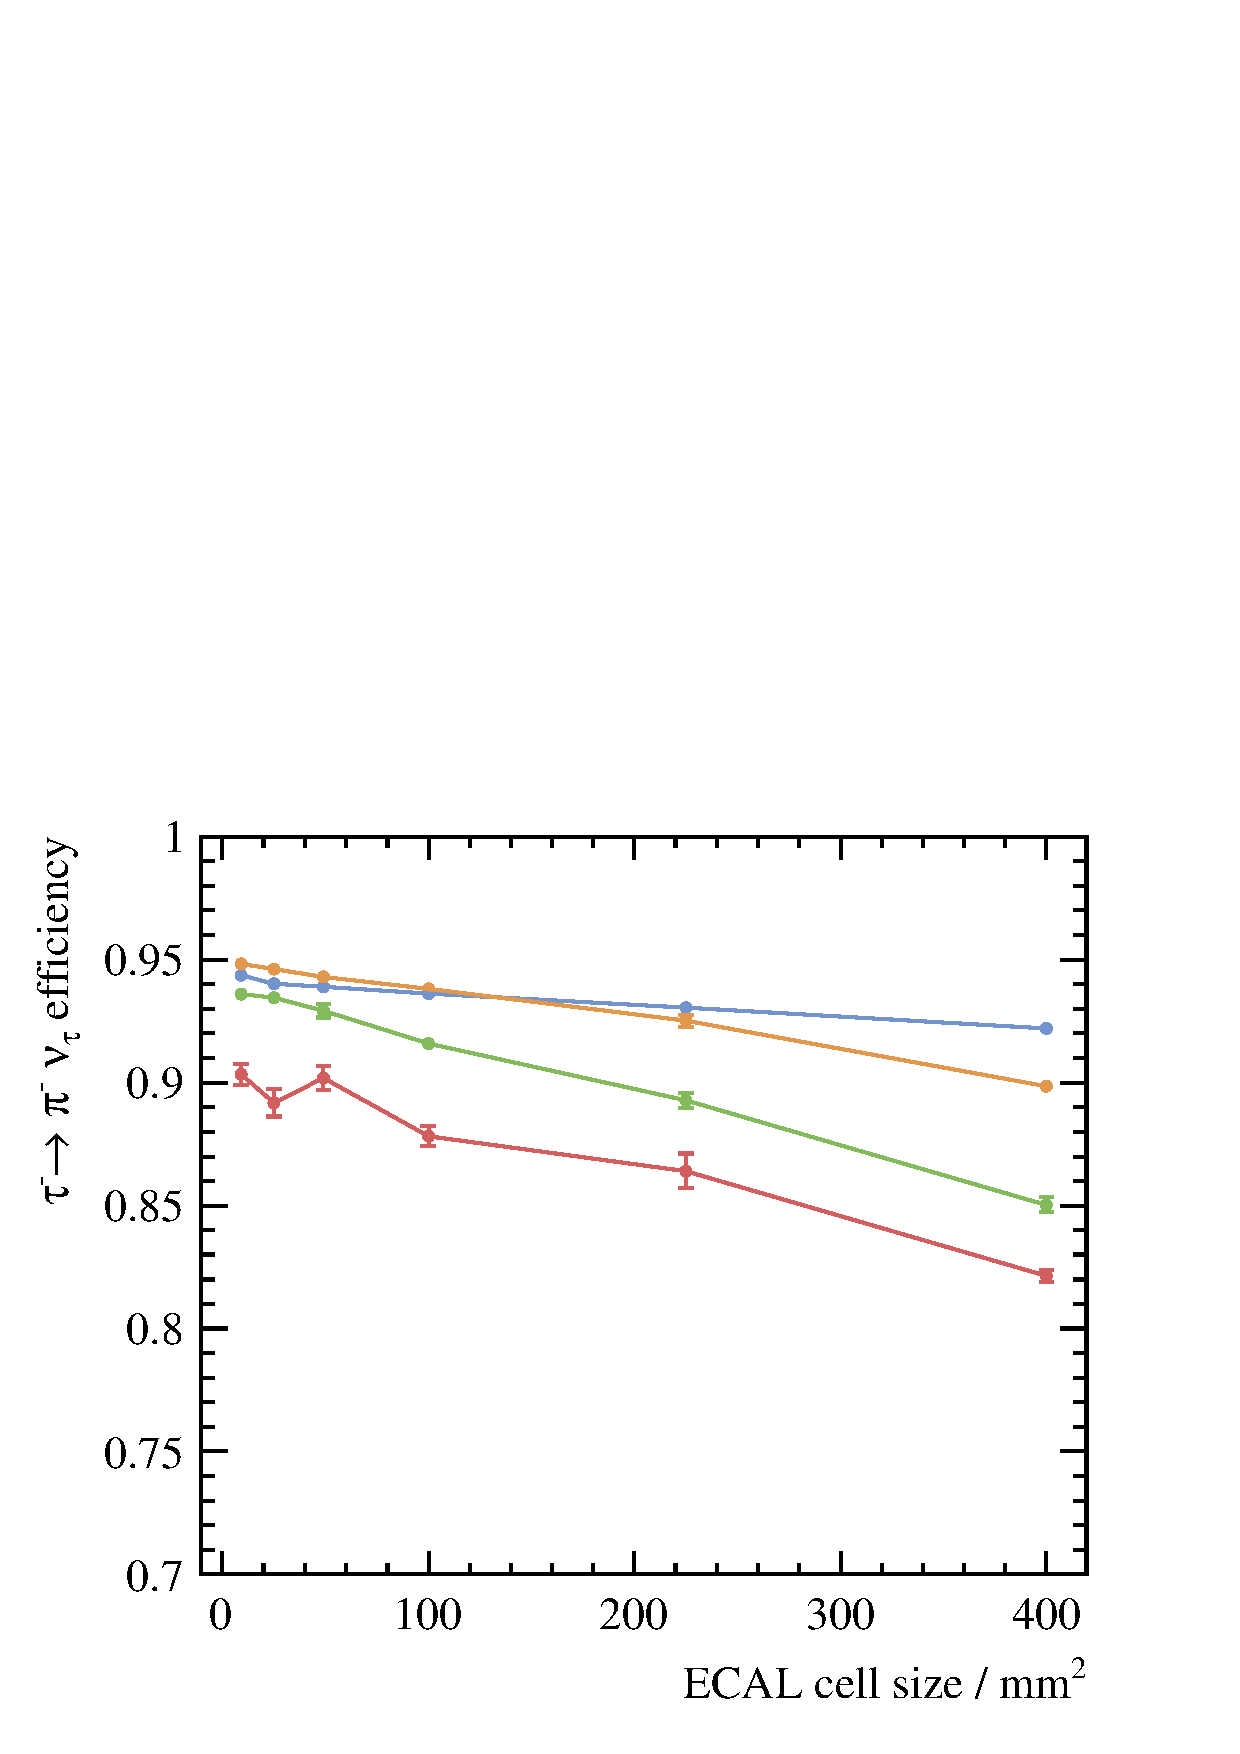
\includegraphics[width=\textwidth]{tau/plots3/decayMode2.pdf}
  \caption{}
  \label{fig:tauDecayMode2}
\end{subfigure}
\begin{subfigure}[b]{0.45\textwidth}
  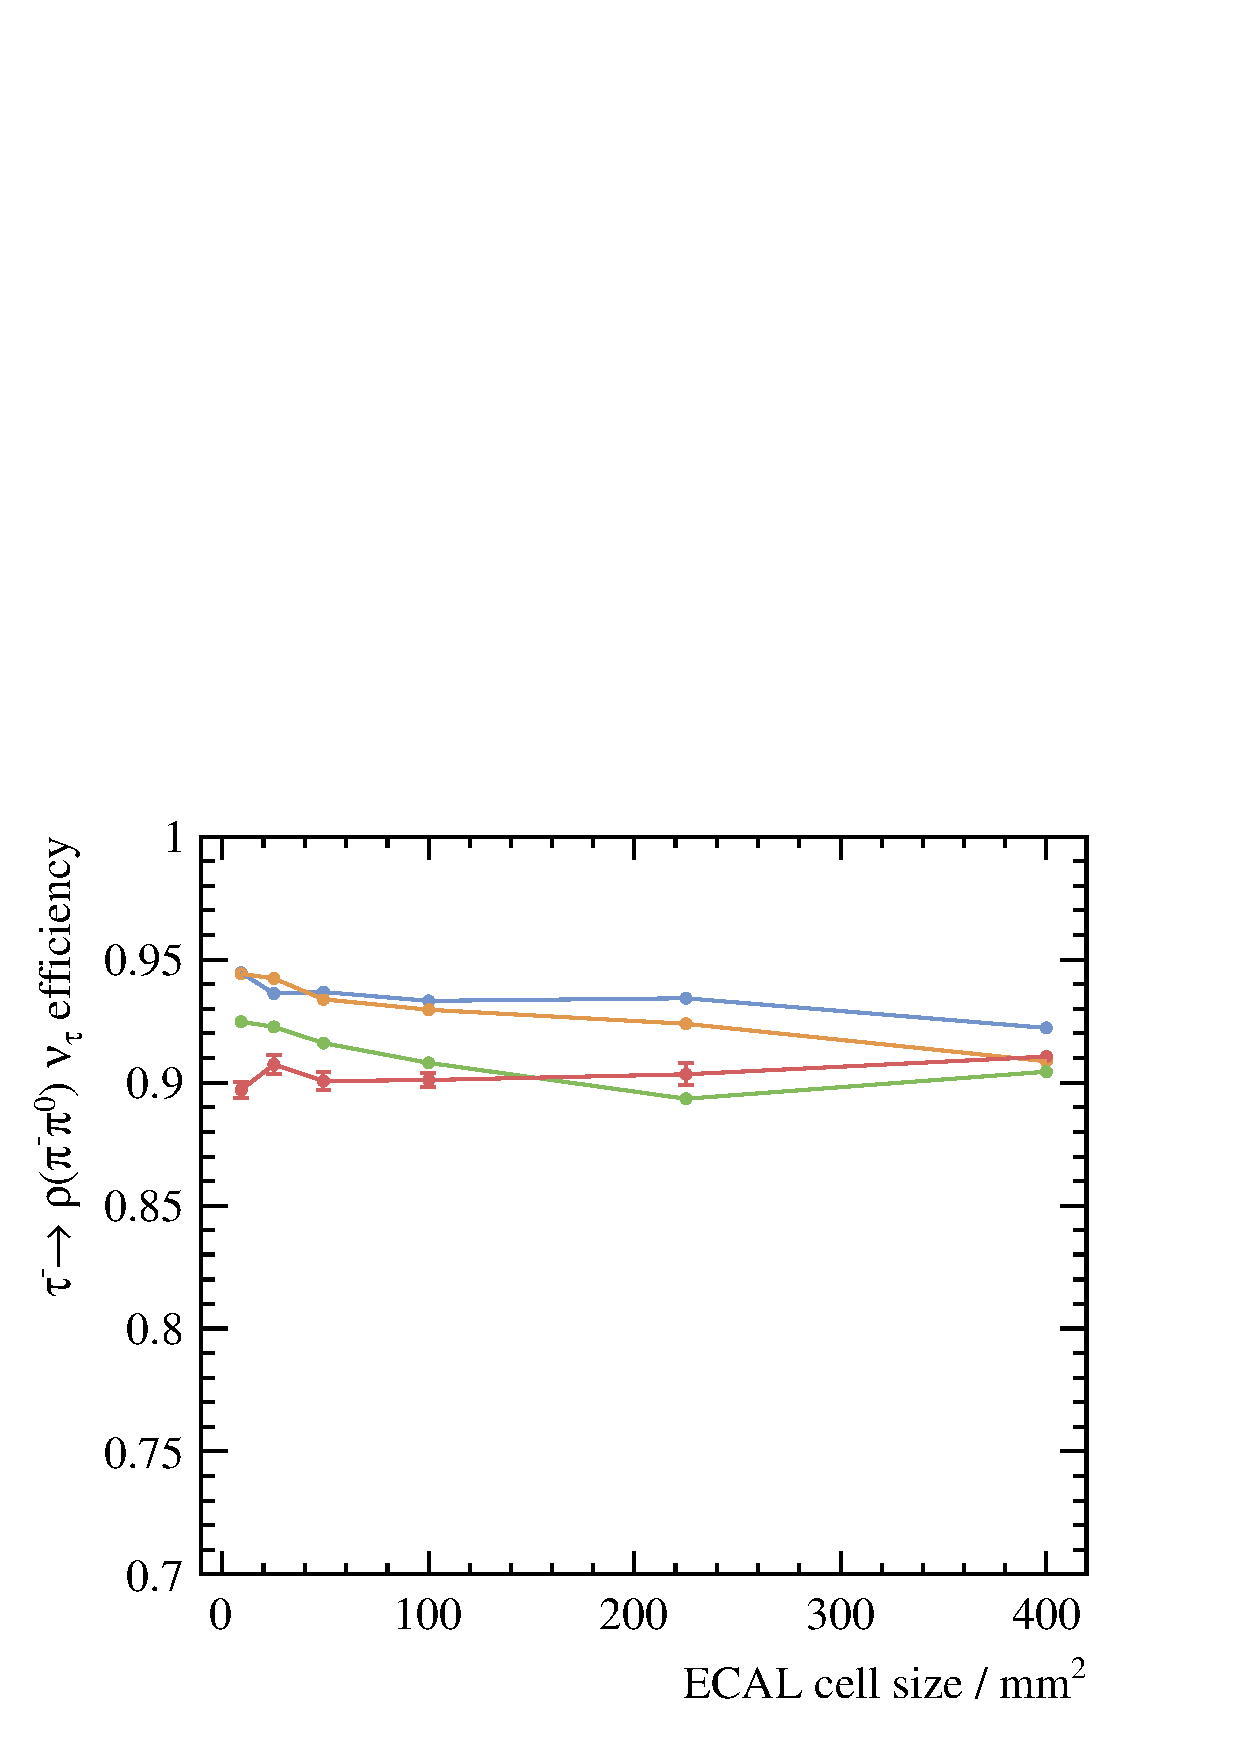
\includegraphics[width=\textwidth]{tau/plots3/decayMode3.pdf}
  \caption{}
  \label{fig:tauDecayMode3}
\end{subfigure}
\begin{subfigure}[b]{0.45\textwidth}
  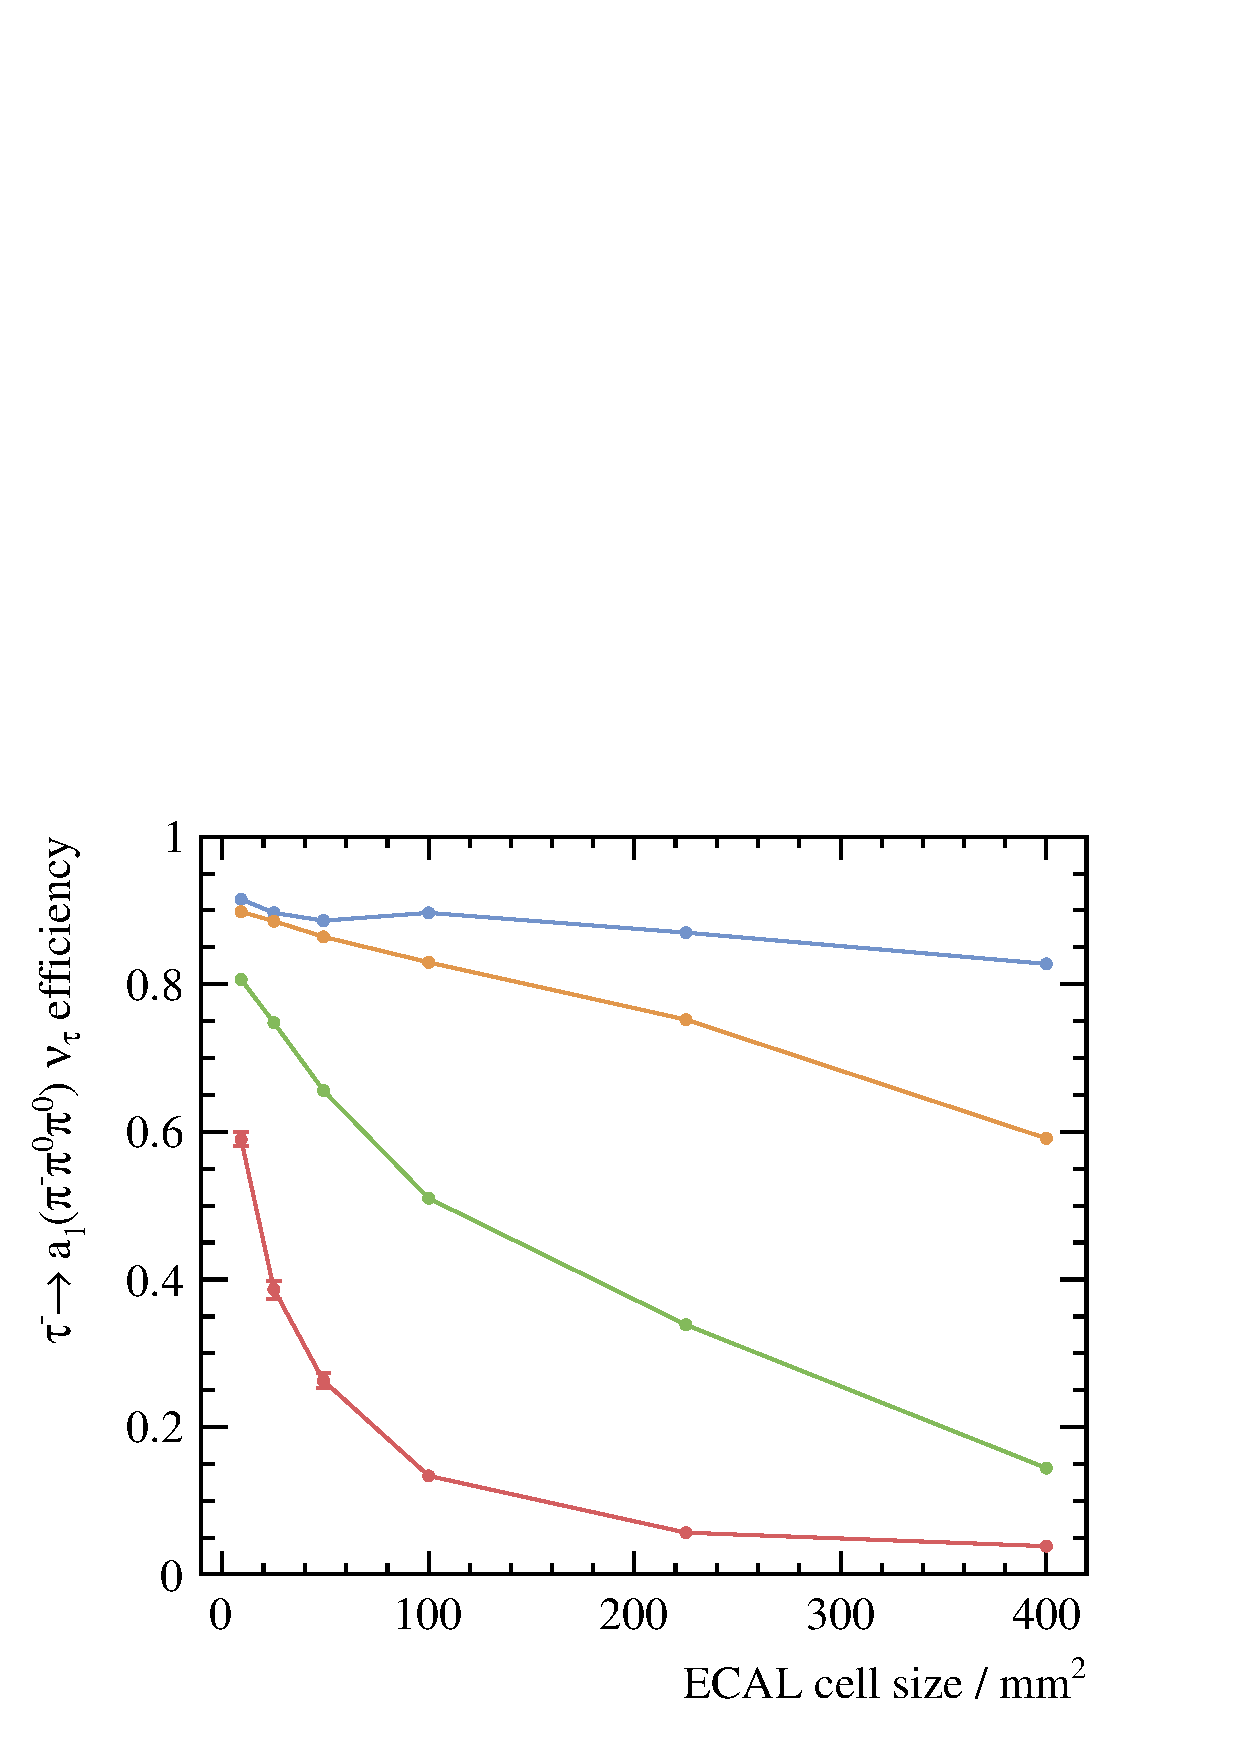
\includegraphics[width=\textwidth]{tau/plots3/decayMode4.pdf}
  \caption{}
  \label{fig:tauDecayMode4}
\end{subfigure}
\begin{subfigure}[b]{0.45\textwidth}
  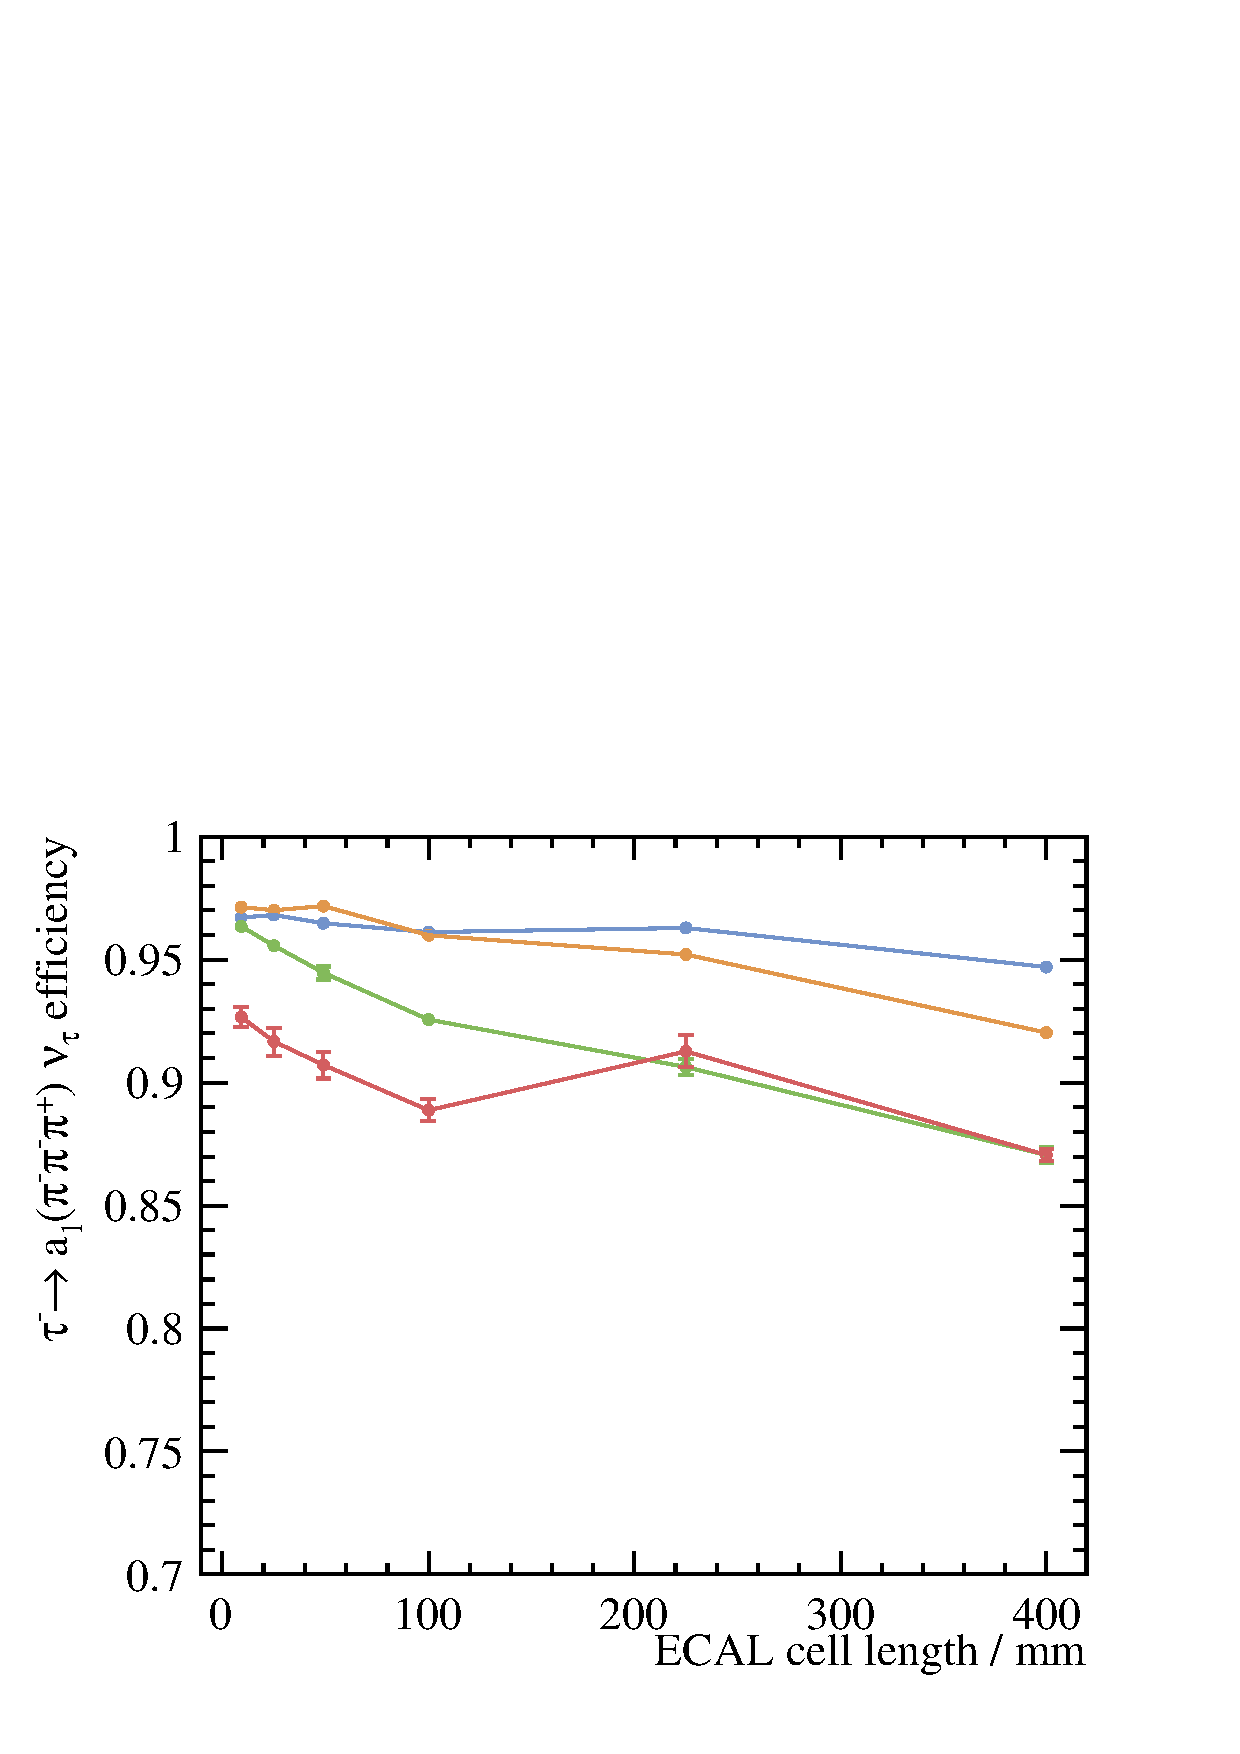
\includegraphics[width=\textwidth]{tau/plots3/decayMode5.pdf}
  \caption{}
  \label{fig:tauDecayMode5}
\end{subfigure}
\begin{subfigure}[b]{0.45\textwidth}
  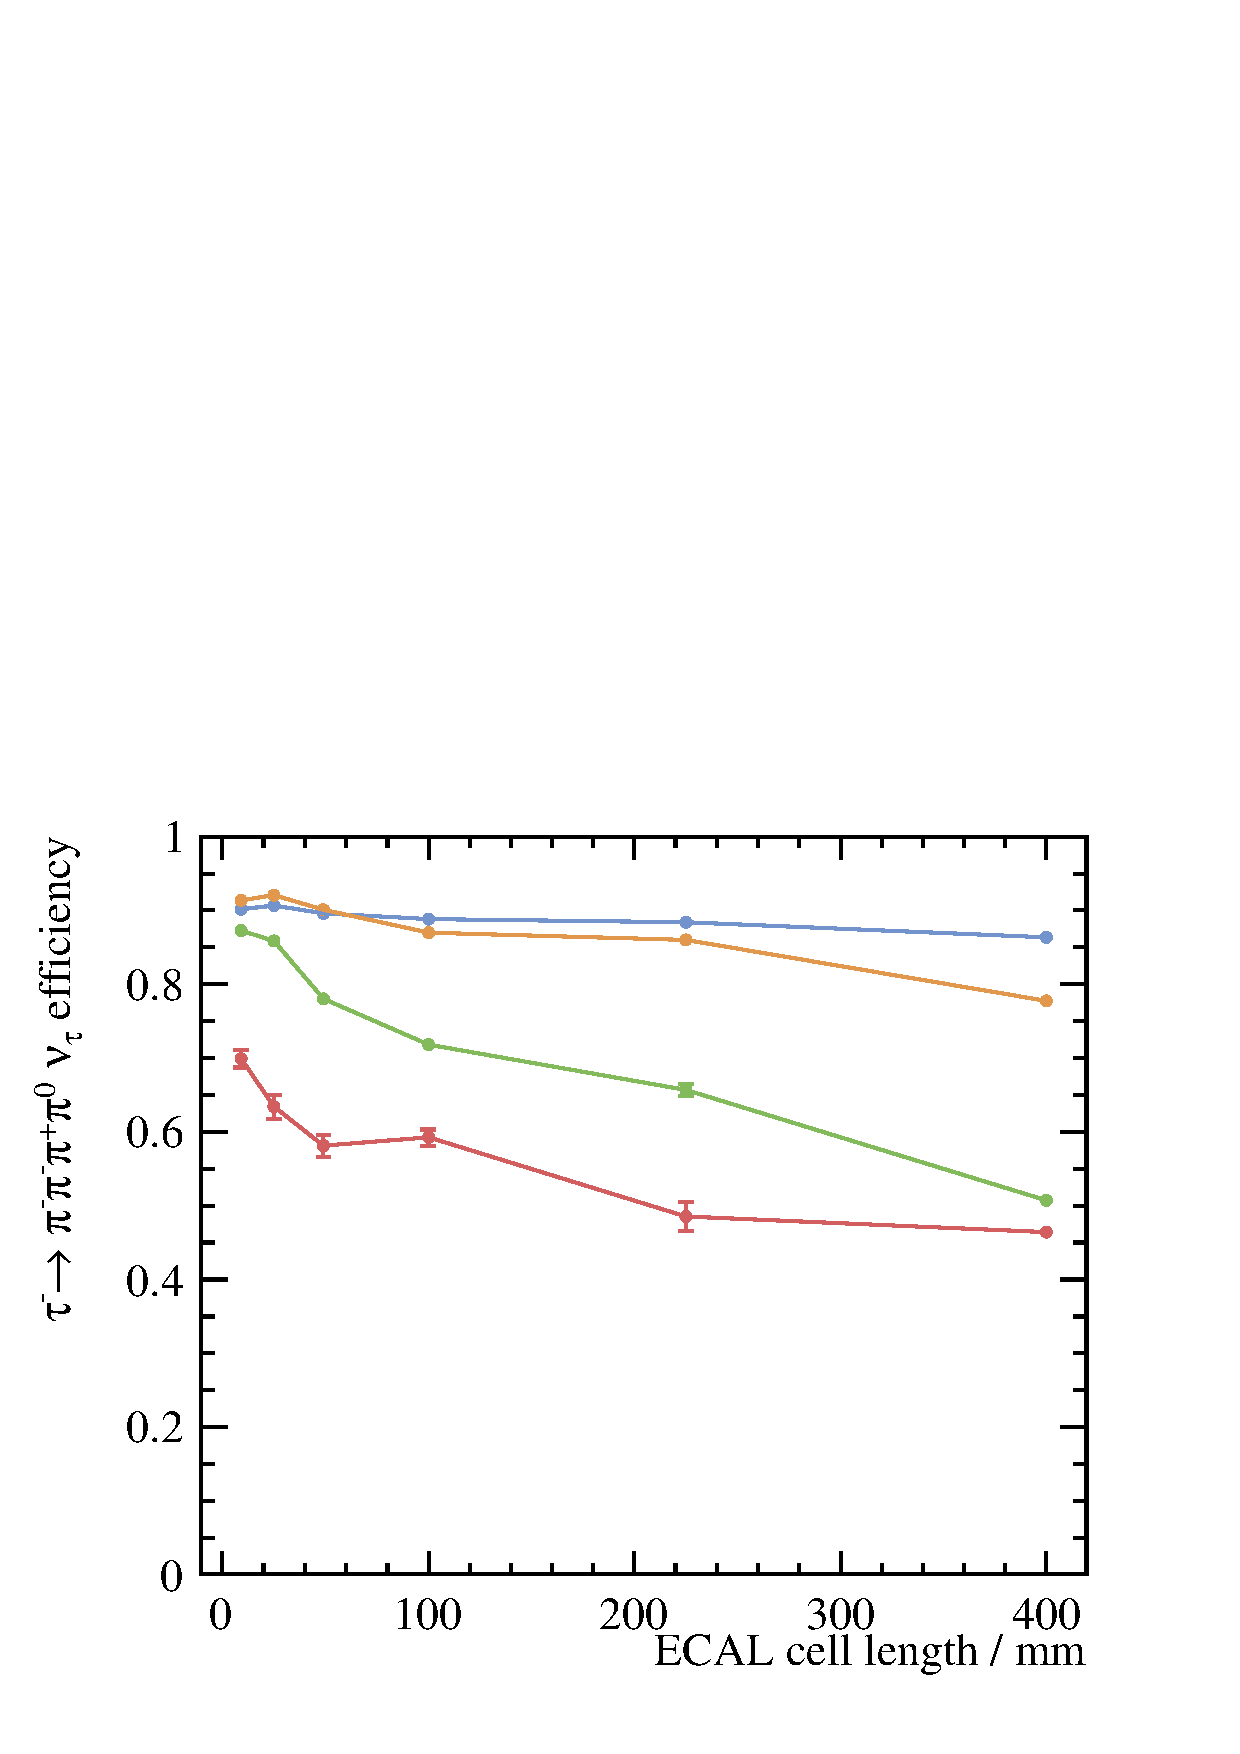
\includegraphics[width=\textwidth]{tau/plots3/decayMode6.pdf}
  \caption{}
  \label{fig:tauDecayMode6}
\end{subfigure}
\begin{subfigure}[b]{0.45\textwidth}
  \includegraphics[width=\textwidth]{tau/plots3/legend.pdf}
  \caption{}
  \label{fig:tauDecayLegend}
\end{subfigure}
\caption[The correct classification efficiency for  tau hadronic decay final states  as a function of the \ECAL square cell sizes]
{
 The correct classification efficiencies for  tau hadronic decay final states  as a function of the \ECAL square cell sizes, using the \ILD detector model with \sqrtS = 100, 200, 500 and 1000\,GeV. \FIGURE{fig:tauDecayMode2}, ~\ref{fig:tauDecayMode3}, ~\ref{fig:tauDecayMode3}, ~\ref{fig:tauDecayMode4},  and ~\ref{fig:tauDecayMode5} show the  \decayPionShort,  \decayRhoShortest, \decayAiPhotonShortest, \decayAiPionShortest, \decayThreePionPhotonShort decay modes, respectively.}
\label{fig:TauPionEfficiency}
\end{figure}


\subsection{Tau hadronic decay correct classification efficiency}

There are two reasons for constructing a single parameter for the overall Tau decay efficiency. First is that multivariate classifier is trained to optimised for the overall classification efficiency. Second is that it is easier to compare the impact of different detector models and different \sqrtS. The choice of the hadronic decay  is because reconstructing hadronic decays is sensitive to the \ECAL cell sizes, which is relevant for this study.

The constructed  Tau hadronic decay correct classification efficiency, \tauHad, is a weighted classification efficiency for all hadronic decay modes:
\begin{equation}
\label{eq:had}
\tauHad = \frac{\sum_{i}^5 {Br}_{i}\varepsilon_{i}}{\sum_{i}^5 {Br}_{i}}  \,,
\end{equation}
where $Br_{i}$ is the branching fraction of the hadronic decay mode $i$  after the generator level cut (\Section{sec:tauPreSel}). $\varepsilon_{i}$ is the correct reconstruction efficiency of the decay mode $i$, and $i$ is summing over five tau hadronic decay modes.

\FIGURE{fig:TauHadronicEfficiency} shows \tauHad as a function of \ECAL cell sizes with different \sqrtS. The general trend for the \tauHad is that \tauHad decreases with increase of \sqrtS and increase of \ECAL cell sizes for the same reasons stated in the previous section. As the \sqrtS increases, tau decay products are boosted and it is challenging to separate identical decay products. Similarly,  increasing \ECAL cell sizes makes particle separation more difficult.

For \tauHad at \rootSGeV{100}, the efficiency decreases from 94\% at 3\,mm cell size, to 91\% at 20\,mm cell size. The decrease is approximately proportional to the increase in the cell size.

For \tauHad at \rootSGeV{200}, the efficiency decreases from 94\% at 3\,mm cell size, to 86\% at 20\,mm cell size.
%There is a large decrease from 15\,mm to 20\,mm cell size.

For \tauHad at \rootSGeV{500}, the efficiency decreases from 92\% at 3\,mm cell size, to 78\% at 20\,mm cell size. Most significant decrease occurs at this \sqrtS.

For \tauHad at \rootSGeV{1000}, the efficiency decreases from 85\% at 3\,mm cell size, to 75\% at 20\,mm cell size.
%From 10\,mm cell size onwards, the \tauHad decrease slows down.

The increase in \ECAL cell sizes has a larger impact on high \sqrtS. With decay products spatially close at high \sqrtS, it is more beneficial to have a smaller \ECAL cell size to reconstruct individual particle.

\begin{figure}[htbp]
\centering % \begin{center}/\end{center} takes some additional vertical space
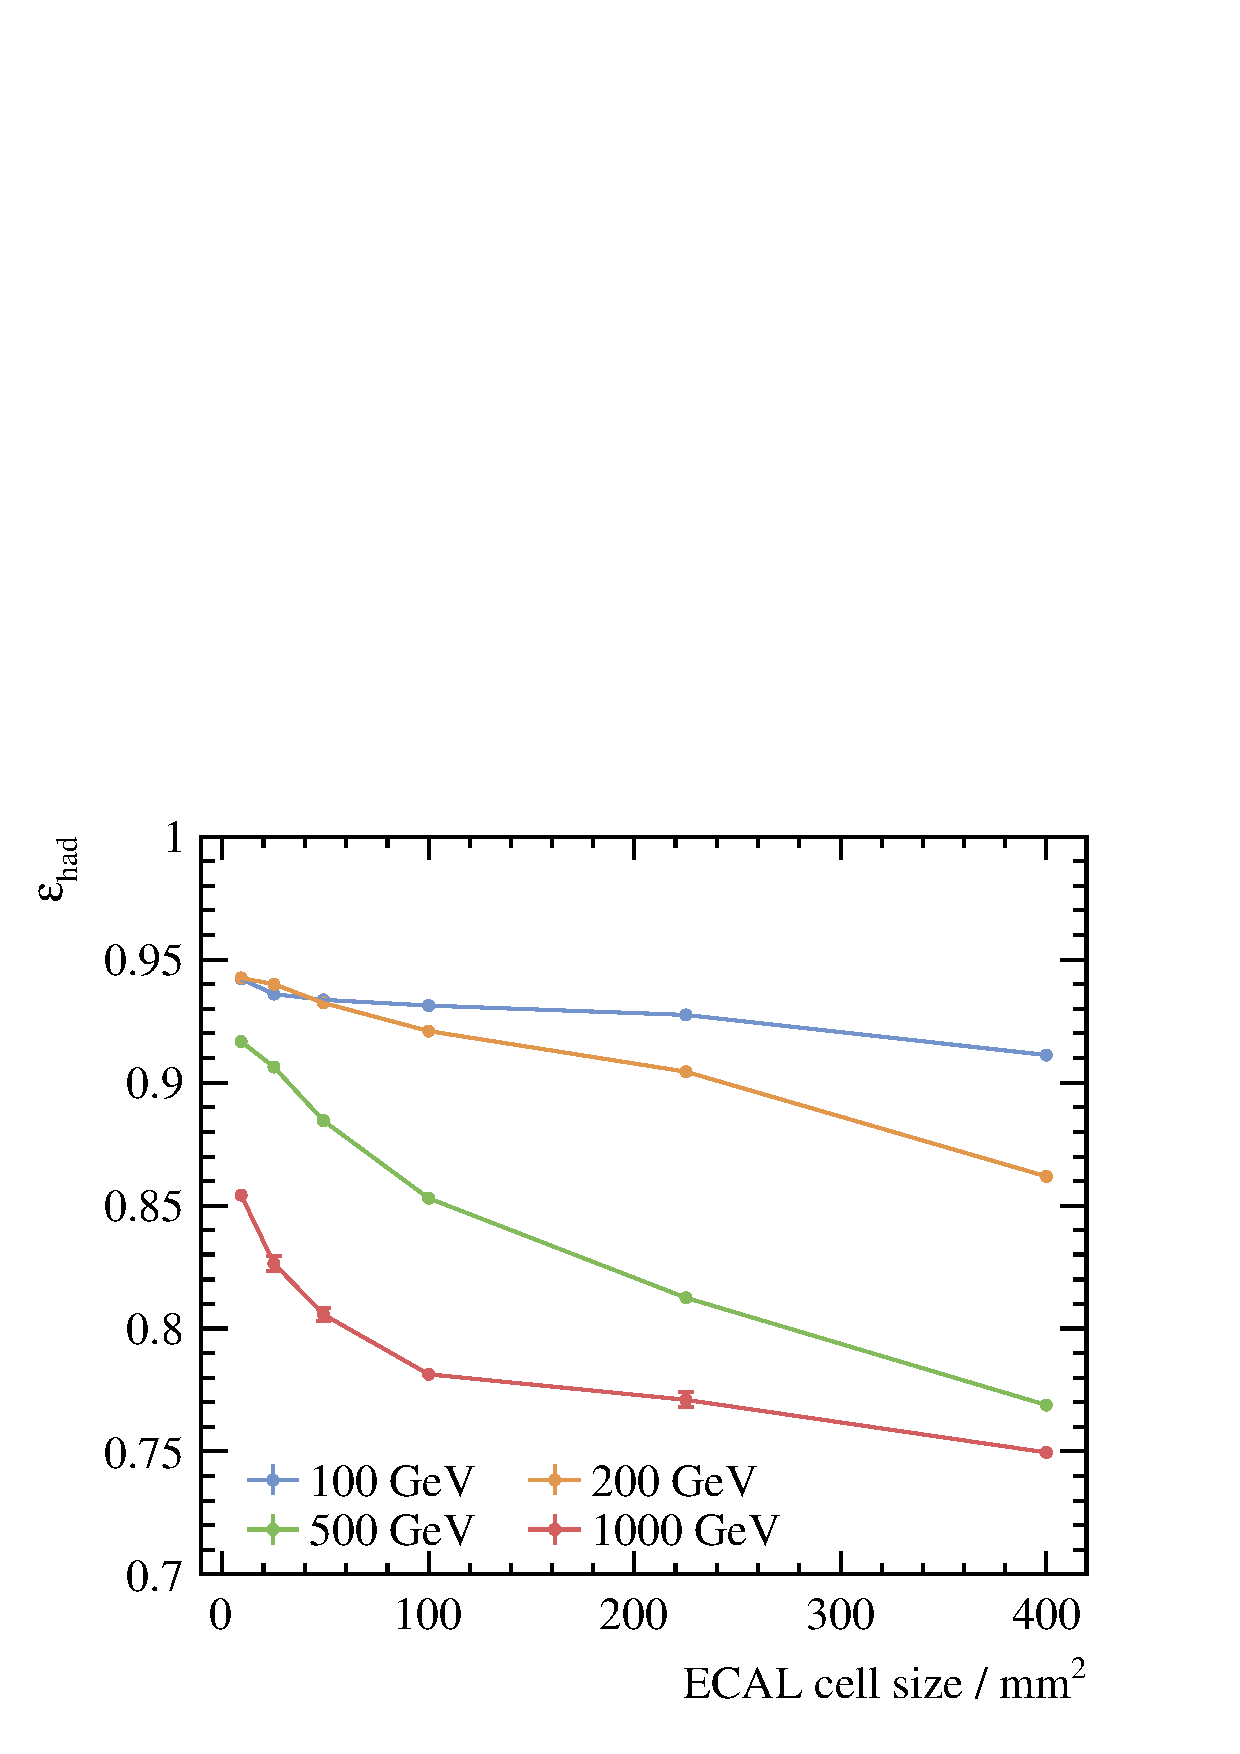
\includegraphics[width=.45\textwidth]{tau/plots3/hadronicEff.pdf}
\caption[The tau hadronic decay efficiency as a function of  the \ECAL cell sizes at different \sqrtS with the nominal \ILD detector model.]
{The tau hadronic decay efficiency, \tauHad, as a function of  the \ECAL cell sizes at different \sqrtS with the nominal \ILD detector model. The blue, orange, green and red lines are representing the \sqrtS = 100, 200, 500 and 1000\,GeV respectively.}
\label{fig:TauHadronicEfficiency}
\end{figure}


\section{Separate \PHiggs from \PZ with tau pair decay}
\label{sec:tauHZ}
\PHiggs can be separated from  \PZ using  tau pair decay channel.  The difference in the spin of the boson reflects in the different polarisation correlation of the tau pair. By extracting the polarisation correlation, parent bosons can be separated. A proof-of-principle analysis is presented to demonstrate the physics usage of the tau decay mode classification, motivated by theoretical studies such as in \cite{Bullock:1991my}. The theoretical motivation is described in \Section{sec:theoryTauPair}. The subsequent sections discuss the ability to reconstruct the polarisation correlation of the \PZ using tau pair decay, and to match with the truth information.

The analysis largely follows the same procedure for the tau decay mode classification. Differences are highlighted in sections below.

The channel is \HepProcess{\Pep \Pem \to \PZ \PZ}, where one \PZ decays hadronically and the other \PZ decays to a tau lepton pair. The samples were generated at \rootSGeV{350} without \ISR contribution for this proof-of-principle study.

\subsection{Event pre-selection}

Same seven tau decay modes in \Section{sec:tauDecayModes} are studied. The \tauToPion decay mode is used to demonstrate tau pair polarisation correlation.

The event pre-selection is similar to that in \Section{sec:tauPreSel}. The cut on the visible energy of decay products is not used because a large fraction of \ZToTauTau events where \tauToPion have two low-energy \Ppipm. Therefore, the cut on the visible energy of decay products would bias the distribution.


\subsection{Identify tau pairs}

The final state of \HepProcess{\Pep \Pem \to \PZ \PZ} channel contains two tau leptons and two quark jets. Therefore, tau decay products can either found by direct tau searching, or by finding two jets and working out the recoil. If a tau lepton decays to a few particles, then the direct tau searching would work. If a tau lepton decays to many particles, finding tau decay products as a jet has a better performance. Here two approaches are combined for the best tau pair identification.

\subsubsection{Direct tau search}
Tau finder processer, \BonoTauFinder, is developed by the author, which is a modified version from the one in \Section{sec:doubleHiggsBonoTauFinder}. The basic idea is to find tau decay products consistent with decay topologies, and require the decay products to be isolated from rest of particles in an event. Parameters chosen are loose to find as many as possible tau candidates. The filtering of the candidates is via kinematic constraints.

The modified \BonoTauFinder works as following. Low \pT are not considered. A seed particle is chosen and a search cone is formed around the seed, which requires one or three tracks with the search cone invariant mass less than 3\,GeV. The isolation criteria states that the opening angle between the search cone  and the $2^{nd}$ closest track is larger than 0.6\,rad. If all criterion are satisfied,  the search cone with the tau seed is identified as a tau lepton.

\begin{table}[!htbp]
\begin{tabular}{lr}
\hline
\hline
Modified \BonoTauFinder  & Selection \\
\hline
Veto low \pT (GeV) &  $\pT < 0.5$\\
Seed particle (GeV) & $\pT > 1$ \\
Maximum search cone opening angle (rad) & $\theta_S \leqslant \cos^{-1}(0.99)$\\
Tau candidate rejection & $N_{X^+} \neq 1,3$, $m_{PFO} > 3$   \\
Isolation (rad)& $\theta_{cone,2^{nd}X^+} > 0.6$\\
\hline
\hline
\end{tabular}
\caption
{Optimised parameters of modified \BonoTauFinder.}
\label{tab:tauBonoTauFinderProcessor}
\end{table}

\subsubsection{Jet clustering}

Tau hadronically decay can be also identified as a small jet. Durham algorithm \cite{Catani:1991hj} was used to jet clustering, also known as \ee \kt algorithm. (see \Section{sec:pandoraJetDurham}). The jet algorithm runs in the exclusive mode to find four jets.

\subsubsection{Select tau candidates}

The best tau pair candidates are selected using kinematic constraints. Half of \sqrtS is in the \PZ. The invariant mass of two quarks from \PZ should be close to \PZ mass. Therefore, the minimisation function is
\begin{equation}
\chi^2 = \frac{\parenths{m_{\Pquark\Pquark} - m_{\PZ}}^2}{\sigma_{m_{\Pquark\Pquark}}^2} + \frac{\parenths{E_{\Pquark\Pquark} - \frac{\sqrtS}{2}}^2}{\sigma_{E_{\Pquark\Pquark}}^2},
\label{eq:tauMinimiser}
\end{equation}
where $m_{\PZ}$ is the mass of \PZ from reference \cite{Agashe:2014kda}. $\sigma_{m_{\Pquark\Pquark}}$ and $\sigma_{E_{\Pquark\Pquark}}$ are the reconstructed resolution of mass and energy of the \PZ, respectively.  $m_{\Pquark\Pquark}$ and  $E_{\Pquark\Pquark}$ are defined differently for the direct tau searching and the jet clustering method. For the direct tau search method, $m_{\Pquark\Pquark}$ and  $E_{\Pquark\Pquark}$ are defined as the recoil against two tau candidates, assuming collision at \sqrtS, iterating over all  tau candidates. For the jet clustering method,  $m_{\Pquark\Pquark}$ and  $E_{\Pquark\Pquark}$ are defined as the mass and energy of two jets, iterating over all possible jets.

The $\chi^2$ minimiser is repeated for the direct tau search and the jet clustering method. Each method produces a best tau pair candidate. Hence two tau pair candidates are obtained. To find the over best tau candidate, a set of conditions is used. If best tau pair candidates for both methods satisfy the kinematic constraint:
\begin{equation}
\absOf{m_{\Pquark\Pquark} - m_{\PZ}} < \sigma_{m_{\Pquark\Pquark}}\ , \absOf{E_{\Pquark\Pquark} - \frac{\sqrtS}{2}} < \sigma_{E_{\Pquark\Pquark}},
\label{eq:tauMinimiserSelector}
\end{equation}
the pair with smallest $\chi^2$ is chosen.

If only one candidate satisfies the constraint in \Equation{eq:tauMinimiserSelector}, that candidate is chosen. If none of the candidates satisfies the constraint, and if one jet from the jet clustering is close to the beam pipe and there are exactly two tau leptons from \BonoTauFinder, then these two tau leptons are chosen. This is because if one jet is close to the beam pipe, it is likely that some particles are undetected, which leads to a failure in the kinematic constraint. Lastly, if all conditions above are not satisfied, two smallest jets by number of \PFOs are chosen to be tau leptons decay products.

\subsubsection{Boost to \PZ decay rest frame}

To use the tau decay mode classifier, it is necessary to know the tau lepton energy before decaying. For the channel \PZ decaying to a tau pair, the tau energy can be calculated in \PZ decay rest frame, which is half of the \PZ energy. To calculate the energies of tau decay products in the rest frame, the decay products need to be boosted to the rest frame, which requires the \fourMomentum of the \PZ, the tau pair system.

The previous section describes the method to identify the tau pair decay products. The \fourMomentum of the \PZ decaying to tau pair is calculated from the recoil of non tau decay products:
\begin{equation}
p^{\mu}_{\Ptau\Ptau} =
  \begin{pmatrix}
    \sqrtS\\   \sqrtS\times\sin\parenths{\theta_{beam}}\\  0   \\       0 \\
  \end{pmatrix}
  - \sum_{i}^{non-\Ptau}p^{\mu}_{i},
\end{equation}
where $\theta_{beam}$ is the beam crossing angle. Index $i$ is summing over all non tau decay \PFOs. Extra kinematic constraint fixes the energy of the $p^{\mu}_{\Ptau\Ptau}$ to be half of \sqrtS:
\begin{equation}
p^{\mu}_{\Ptau\Ptau,correct} \equiv p^{\mu}_{\Ptau\Ptau} \times \frac{\frac{1}{2}\sqrtS}{E_{\Ptau\Ptau}}.
\end{equation}
$p^{\mu}_{\Ptau\Ptau,correct} $ is used as the boost vector to boost tau decay products in the rest frame. The calculation of the variables for the MVA classifier are preformed in the rest frame.

\subsection{Variables}

Variables for the MVA classifier are largely the same as the ones in \Table{tab:tauVaraibles}. Variables regarding EM shower profiles, calorimeter hit information and track information are not used (last three rows in \Table{tab:tauVaraibles}) as the study focus on the overall tau decay mode separation. Also for the computational reason, it was not feasible to use these variables for the MVA. \Pep and \Ppiplus separation could be improved if these extra variables are included.


\subsection{Multivariate analysis}

Half of the sample is used to train the multivariate classifier,  which follows the procedure in  \Section{sec:tauMVA}. In the applying stage, \tauToPion decay mode is selected with additional criteria that at least one \Ppipm is identified in the tau decay products.

\subsection{Result}

\FIGURE{fig:TauSpin2D} shows the two-dimensional plot of tau pair polarisation correlations from \PZ decay, using \tauToPion decay mode. The energy fractions are the appreciate kinematic variables, motivated in \Section{sec:theoryTauPair}. \FIGURE{fig:TauSpin2DMC} shows the distribution using the truth information. \FIGURE{fig:TauSpin2Dreco} shows the distribution using full detector simulation. In the \ZToTauTau decays, an energetic \Ppipm is likely to be associated with an energetic \Ppipm, shown in both \Figure{fig:TauSpin2DMC} and \Figure{fig:TauSpin2Dreco}. Comparing two figures, some events in the top right quadrant, resembling both \Ppipm being energetic, are not reconstructed correctly. This is due to the incorrect identification of the tau pair decay products.

This proof-of-principle analysis shows the tau polarisation correlations with \ZToTauTau decay where \tauToPion can be observed. With a similar study of \HiggsToTauTau, such  the tau polarisation correlations can be used to sperate \PHiggs from \PZ.


\begin{figure}[htbp]
\centering % \begin{center}/\end{center} takes some additional vertical space
\begin{subfigure}[b]{0.45\textwidth}
  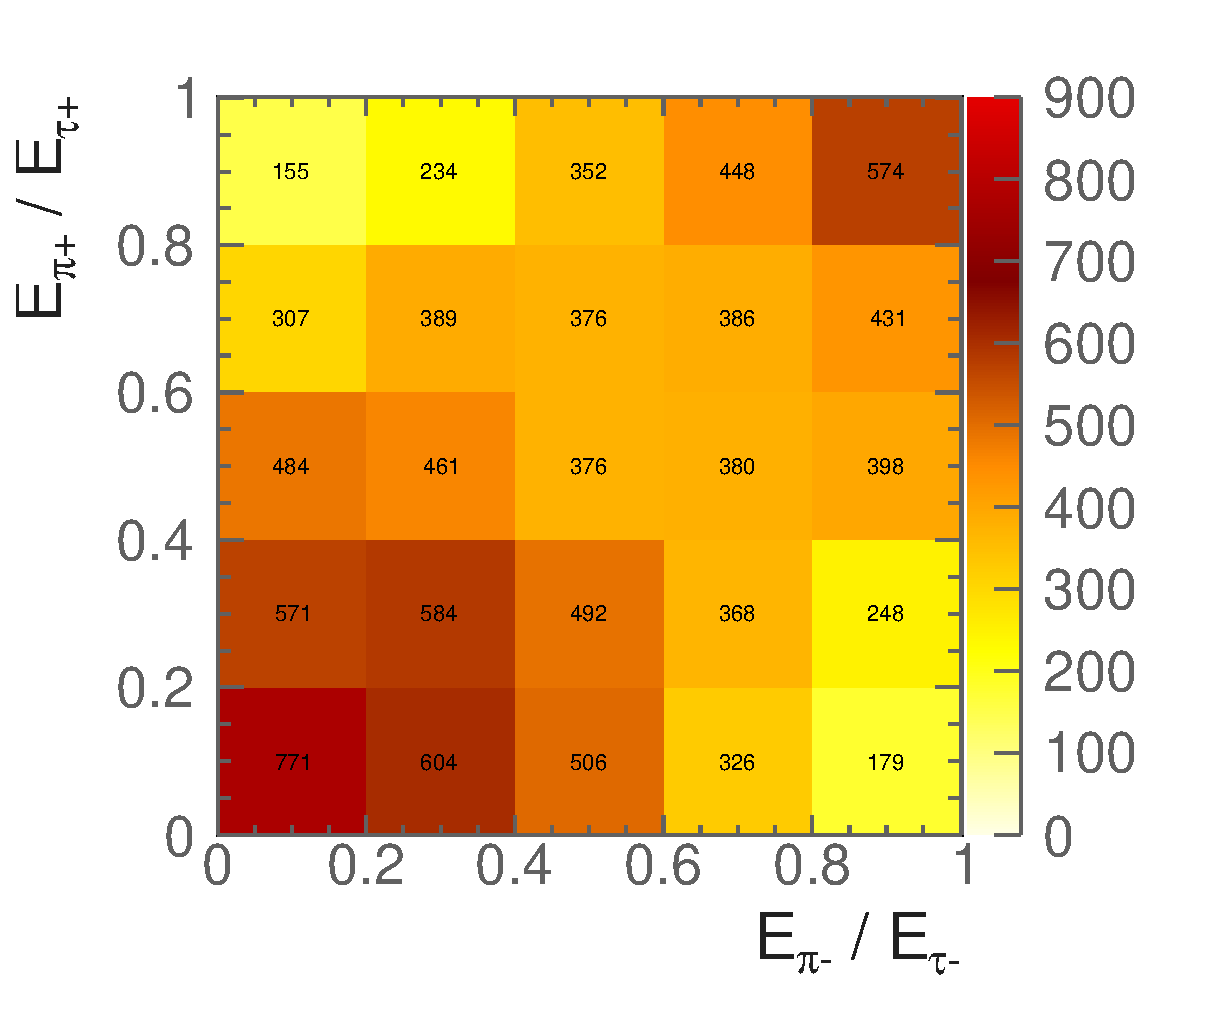
\includegraphics[width=\textwidth]{tau/NoTimeAnalysis/2DMC}
  \caption{Truth info.}
  \label{fig:TauSpin2DMC}
\end{subfigure}
\begin{subfigure}[b]{0.45\textwidth}
  \includegraphics[width=\textwidth]{tau/NoTimeAnalysis/2Dreco}
  \caption{Simulated}
  \label{fig:TauSpin2Dreco}
\end{subfigure}
\caption
{Two-dimensional plot of tau pair polarisation correlations from \PZ decay, using \tauToPion decay mode.}
\label{fig:TauSpin2D}
\end{figure}
\begin{comment}
\begin{figure}[htbp]
\centering % \begin{center}/\end{center} takes some additional vertical space
\begin{subfigure}[b]{0.45\textwidth}
  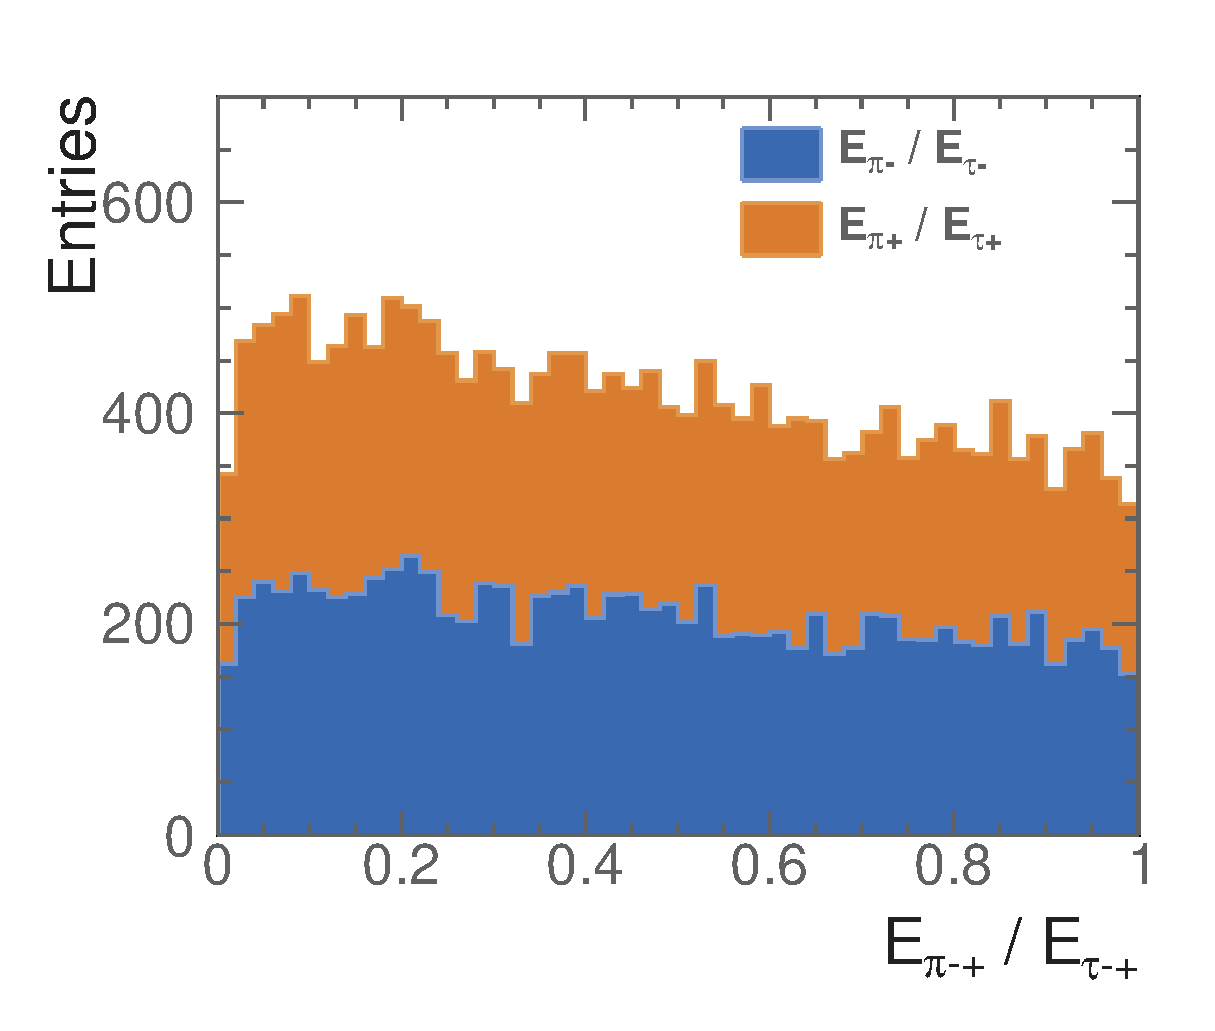
\includegraphics[width=\textwidth]{tau/NoTimeAnalysis/1DMC}
  \caption{Truth info.}
  \label{fig:TauSpin1DMC}
\end{subfigure}
\begin{subfigure}[b]{0.45\textwidth}
  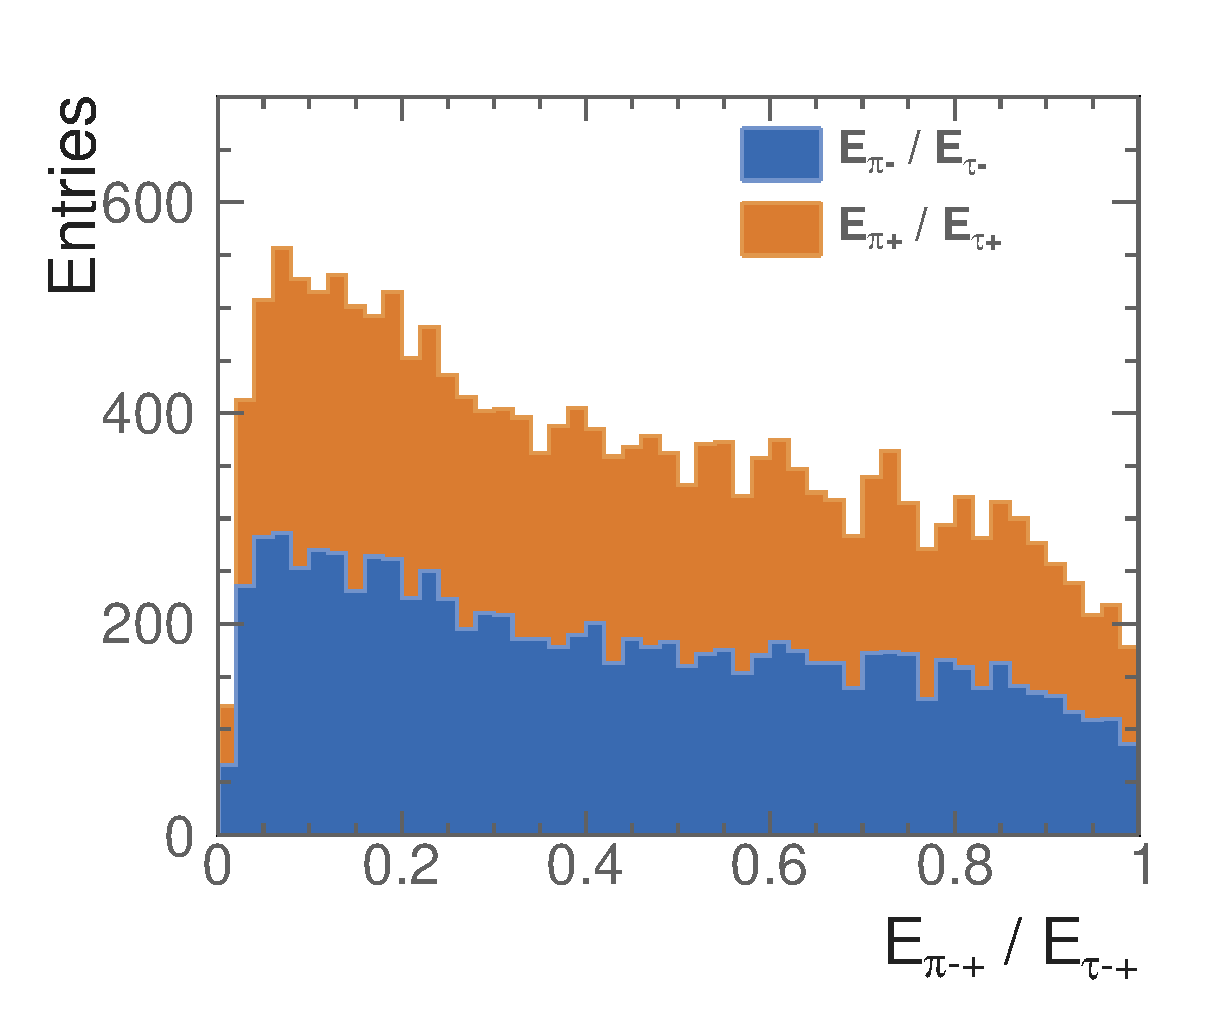
\includegraphics[width=\textwidth]{tau/NoTimeAnalysis/1DrecoNoOverflow}
  \caption{Reconstructed}
  \label{fig:TauSpin1Dreco}
\end{subfigure}
\caption[One-dimensional plot of spin correlations of the tau lepton pair from \PZ decay, using \decayPionShort decay mode.]
{One-dimensional plot of spin correlations of the tau lepton pair from \PZ decay, using \decayPionShort decay mode.}
\label{fig:TauSpin1D}
\end{figure}

\end{comment} 